\chapter{Probability} \label{Sec:probability}

In this chapter, we turn our attention to the ideas of probability and randomness. This is important because in many physical systems we do have true randomness because of the laws of quantum mechanics. Individual particle interactions, for example can only be described probabilistically in the sense that when and what interacts a particle undergoes is inherently random. Furthermore, we often apply the ideas of probability to systems that are essentially deterministic, but appear random because of uncertainties resulting from our limited information of a particular system. For example, the failure time of a machine could be predicted if we fully understood the physics of every component of that machine at all points in time. Because this is not practical, we often use a mathematical model involving randomness to analyze failure rates and overall consequences of such systems. Furthermore, the ideas of probability theory are used strongly in many algorithms related to data analytics or machine learning in that they use large amounts of data to make inferences about particular systems with many unknowns.



%%%%%%%%%%%%%%%%%%%%%%%%%%%%%%%%%%%%%%%%%%%%%%%%%%%%%%%%%%%%%%%%%%%%%%%%%%%%%%%%%%%%%%%%%%%%%%%
%%%%%%%%%%%%%%%%%%%%%%%%%%%%%%%%%%%%%%%%%%%%%%%%%%%%%%%%%%%%%%%%%%%%%%%%%%%%%%%%%%%%%%%%%%%%%%%
\section{Basic Concepts}

%%%%%%%%%%%%%%%%%%%%%%%%%%%%%%%%%%%%%%%%%%%%%%%%%%%%%%%%%%%%%%%%%%%%%%%%%%%%%%%%%%%%%%%%%%%%%%%
\subsection{Interpretations of Probability}
Before going into the discussion of the mathematics of probability theory, let's pause and very briefly discuss the meaning of probability. There are two major philosophical interpretations of the concept of probability. 

The first is the \emph{frequentist} interpretation. The frequentist interpretations views probability, as the name implies, as measuring the frequency of a given random event having a particular outcome. For example, suppose we measure the number of radioactive decays from a particular sample in a given time window. Because radioactive decay is inherently a random process, and each time we perform the experiment we expect to get a different result. If we repeat the experiment numerous times, we can make inferences about how likely it is to have a particular number or range of counts in a given time interval. 

The second major philosophical interpretation of probability is the \emph{Bayesian} interpretation. The Bayesian approach to probability views the concept as measuring the degree of belief or logical support for a given hypothesis. For example, suppose we wish to decide whether we should perform an expensive and time consuming preventative maintenance procedure in a nuclear power plant before the next scheduled outage. We could assign a relative probability based on our degree of believe whether equipment would fail and therefore maintenance would be required. We could assign this prior probability, based on, for example, past performance data at this or other nuclear power plants or even a subjective guess. Suppose we then collect information from engineers performing inspections on various components throughout the plant and obtain data from various sensors throughout the plant that could indicate potentially off-normal conditions. Based on the results of these inspections and sensor data we can refine our degree of belief as to whether the unplanned outage for maintenance is required.

Both interpretations of probability are valid and useful in their own contexts. There is come conflict in terms of how to make inference and decision making, but largely we will ignore these issues in this text and focus on the general concepts. 

%%%%%%%%%%%%%%%%%%%%%%%%%%%%%%%%%%%%%%%%%%%%%%%%%%%%%%%%%%%%%%%%%%%%%%%%%%%%%%%%%%%%%%%%%%%%%%%
\subsection{Random Events}

To begin our discussion, we need to define the concept of an event. An event is a set of possible outcomes that have a defined probability. Let $A$ be a particular outcome and $P(A)$ be the probability that outcome $A$ occurs. A few examples of events and outcomes are as follows:
\begin{itemize}
  \item Rolling two dice and getting a particular total;
  \item A piece of equipment in a laboratory fails before a replacement arrives;
  \item A sensor reading in a nuclear power plant is accurate within a particular range;
  \item An engineer has performed a calculation without any mistakes.
\end{itemize}
Probabilities must be assigned so that for any event:
\begin{align}
  0 \le P(A) \le 1 .
\end{align}
An event also has a complementary event $\overline{A}$, which is the oppose of the event. If the event is complimentary, then we have
\begin{align}
  P(A) + P(\overline{A}) = 1.
\end{align}

We can also have multiple events $A$ and $B$ that may or may not be related. We define that the probability that both $A$ and $B$ occurs as $P(A,B)$. If the events are disjoint or mutually exclusive, we say that $P(A,B) = 0$. Alternatively, we can state that the probability of either $A$ or $B$ occurring is $P(A) + P(B)$. In general, we can state that
\begin{align}
  P( A \cup B ) = P(A) + P(B) - P(A,B) .
\end{align}
In other words, the probability that either $A$ or $B$ occurs is the probability that $A$ occurs (regardless of $B$) plus the probability that $B$ occurs (regardless of $A$) minus the probability that both $A$ and $B$ occur.

If the two events are unrelated, we call them independent and can state that
\begin{align}
  P(A,B) = P(A)P(B), \text{ only if events $A$ and $B$ are independent.}
\end{align}

%%%%%%%%%%%%%%%%%%%%%%%%%%%%%%%%%%%%%%%%%%%%%%%%%%%%%%%%%%%%%%%%%%%%%%%%%%%%%%%%%%%%%%%%%%%%%%%
\subsection{Conditional Probability and Bayes' Theorem}

It is often the case we know a particular event $B$ occurred and we wish to know the probability whether a different event $A$ will occur given that information. We denote this as the conditional probability $P(A|B)$. Examples of this include:
\begin{itemize}
  \item If the first of two die is a 4, what is the probability that the total of two die is at least 6?
  \item If a piece of equipment has failed in the first year of operation, what is the probability that an otherwise identical piece of equipment will fail in its first year?
  \item If two sensors report a reading indicating the condition of a system is normal and a third reports an off-normal condition, what is the probability the system is in a normal condition?
\end{itemize}
If $A$ and $B$ are independent of each other then $P(A|B) = P(A)$, since the outcome $B$ has no impact on how likely $A$ is to occur.

We can also infer the result that
\begin{align}
  P(A) &= P(A|B) P(B) + P(A|\overline{B}) P(\overline{B}) .
\end{align}
This states the probability of event $A$ occurring is equal to the probability of $A$ conditional on event $B$ and $A$ conditional on $B$ not occurring. We can generalize this to the law of total probability. If $B_i$ are disjoint events then:
\begin{align}
  P(A) &= \sum_i P(A|B_i) P(B_i) .
\end{align}


We can relate the joint probability to conditional probability as follows:
\begin{align}
  P(A,B) = P(A|B)P(B) = P(B|A)P(A).
\end{align}
From this we can obtain the result known as Bayes' theorem:
\begin{align}
  P(A|B) = \frac{ P(B|A) P(A) }{ P(B) } .
\end{align}

%%%%%%%%%%%%%%%%%%%%%%%%%%%%%%%%%%%%%%%%%%%%%%%%%%%%%%%%%%%%%%%%%%%%%%%%%%%%%%%%%%%%%%%%%%%%%%%
\subsection{Example: Predicting Pump Failure Based on a Sensor}

As an example of Bayes' theorem, let us consider the event $A$ that a pump in a nuclear power plant is not operating normally, indicated by a degraded flow, and requiring maintenance. Based on operating experience, we know that this brand of pump operates correctly 98\% of the time. Therefore, with no additional information, the best we can do is assert that at any given time, there is a 2\% chance that the pump will not be functioning correctly.

Now suppose we have a pressure sensor attached to the pump that can indicate that the pump is failing through measuring degradation in the flow. Let $B$ be the event that the sensor indicates the flow is not normal. Unfortunately, the sensor itself is a piece of equipment that can become uncalibrated and report inaccurate readings, and this must be taken into account in the analysis. From historical operating experience, the sensor will successfully detect degraded flows 99.5\% of the time. Because the sensor can become miscalibrated with time, it will successfully indicate normal flows only 95\% of the time. This implies that the sensor will fail to report a degraded flow 0.5\% of the time and misreport a normal flow as degraded 5\% of the time. Let event $B$ be the sensor indicating an off-normal flow. Suppose we wish to find the probability that the pump is failing.

From the information, we know that the probability that the pump is indeed failing is 2\%, or
\begin{align}
  P(A) = 0.02. \nonumber
\end{align}
The probability that the sensor indicates an off-normal condition regardless of the condition of the pump can be determined from the provided conditional probabilities. We have
\begin{align}
  P(B) &= P(B|A) P(A) + P(B|\overline{A}) P(\overline{A}) \nonumber \\
       &= 0.995 \times 0.02 + 0.05 \times 0.98  \nonumber \\
       &= 0.0199 + 0.049 = 0.0689 . \nonumber
\end{align}
This equation states the probability that the sensor will indicate a degraded flow is the probability of actually detecting the degraded flow plus the probability of misreporting the normal flow as degraded. Note that this result suggests that more often than not, the sensor indicating an off-normal flow is because of it becoming miscalibrated and not because of a problem with the flow itself.

Using Bayes' theorem, we can calculate the probability that the pump is indeed failing if the sensor indicates an off-normal flow:
\begin{align}
  P(A|B) = \frac{ P(B|A) P(A) }{ P(B) } = \frac{ 0.995 \times 0.02 }{ 0.0689 } = 0.288. \nonumber
\end{align}
Therefore, the sensor indicating that the flow is off-normal only gives us a 28.8\% chance that the pump is actually in need of maintenance. In other words, roughly 7 out of 10 times, we would make the wrong decision as to repair the pump.

Since the impact of the former decision is simply lost revenue from conducting an unnecessary repair, it may be worthwhile to analyze the false negative rate of failing to detect a failing pump. For this we require the probability that the sensor indicates normal flow:
\begin{align}
  P(\overline{B}) &= 1 - 0.0689 = 0.9311 . \nonumber
\end{align}
Using Bayes' theorem we can calculate the probability that the pump is actually failing given that the sensor reports normal conditions. This is
\begin{align}
  P(A|\overline{B}) = \frac{ P(\overline{B}|A) P(A) }{ P(\overline{B}) } = \frac{ 0.005 \times 0.02 }{ 0.9311 } = 1.07\times 10^{-4}. \nonumber
\end{align}
This indicates that the chance of the sensor reporting a normal reading and the pump being in need of maintenance is quite low.


%
%
%P( pump is failing | sensor indicates a failure ) = 
%
%P( sensor indicates a failure | pump is failing ) * P( pump is failing ) / P( sensor indicates a failure )

%%%%%%%%%%%%%%%%%%%%%%%%%%%%%%%%%%%%%%%%%%%%%%%%%%%%%%%%%%%%%%%%%%%%%%%%%%%%%%%%%%%%%%%%%%%%%%%
\subsection{Random Variables}

A random variable is a variable whose values depend on some random process. We usually denote a random variable using a capital letter such as $X$ and indicate a particular value that the random variable can take as the lowercase version $x$. Therefore, we say that random variable $X$ takes on value $x$ with probability $P(X = x)$. Underlying every random variable is a probability distribution function that gives the likelihoods of the random variable $X$ taking on a specific value.

Random variables are either discrete or continuous (or possibly a mixture of discrete and continuous, but we will ignore this case). The equations and methods for analyzing each case are very similar, but have some key differences. In the next section we will analyze discrete random variables and then we will analyze continuous random variables in the section that follows. In these will introduce the concepts of the probability mass/density function and the cumulative distribution function.

%%%%%%%%%%%%%%%%%%%%%%%%%%%%%%%%%%%%%%%%%%%%%%%%%%%%%%%%%%%%%%%%%%%%%%%%%%%%%%%%%%%%%%%%%%%%%%%
%%%%%%%%%%%%%%%%%%%%%%%%%%%%%%%%%%%%%%%%%%%%%%%%%%%%%%%%%%%%%%%%%%%%%%%%%%%%%%%%%%%%%%%%%%%%%%%
\section{Discrete Random Variables}

As the name implies, discrete random variables are permitted to take on a set of possibly infinite discrete values. Examples of discrete random variables are:
\begin{itemize}
  \item The result of a coin flip where heads is given a value of 1 and tails is given a value of 0;
  \item The result of the role of a die, which is the set $\left\{ 1, 2, 3, 4, 5, 6 \right\}$;
  \item The number of unplanned nuclear power plant outages in the US in a given year;
  \item The number of counts measured from a radioactive source in a minute;
  \item The energy of a gamma photon emitted during a radioactive decay (the nuclei have discrete energy levels);
  \item The type of reaction that occurs in a neutron-nucleus interaction: scattering, absorption, fission, etc.
\end{itemize}
A discrete random variable is characterized by a probability mass function or cumulative distribution function. In the context of discrete random variables, both of these are probabilities describing the same information in different ways. For continuous random variables, these quantities are fundamentally different, but we will get into that later.

Note that the outcomes of discrete random variables need not be numbers. A common case in nuclear engineering is determining the particular type of interaction that occurs, e.g., scattering, absorption, or fission. We could (and often do) enumerate these reactions with numbers such as 1, 2, 3, \ldots; however, the numbering is arbitrary and merely useful for mathematical bookkeeping.

In this section, we will introduce the concept of a probability mass function and its partner the cumulative distribution function. We will then provide a couple examples. 

%%%%%%%%%%%%%%%%%%%%%%%%%%%%%%%%%%%%%%%%%%%%%%%%%%%%%%%%%%%%%%%%%%%%%%%%%%%%%%%%%%%%%%%%%%%%%%%
\subsection{Probability Mass Function}

The probability mass function gives the probability that a random variable $X$ takes on a particular value $x$. This is denoted with a lowercase function variable $f$ with a subscript being the random variable as
\begin{align}
  f_X(x) = P( X = x ) .
\end{align}
The probability mass function must satisfy the property that if we sum up the probabilities of all possible events, we get one
\begin{align}
  \sum_{x_i} f_X(x_i) = 1 .
\end{align}
All valid probability mass functions are normalized in this way.

A simple example of a probability mass function is that of the case where we have a six-sided die where all sides have an equal probability; the probability mass function is as follows:
\begin{align}
  f_X(x) = \left\{ \begin{array}{r l}
  \frac{1}{6}, & \quad x \in \left\{ 1, 2, 3, 4, 5, 6 \right\} \\
  0, & \quad \text{otherwise} \\ \end{array} \right. .
\end{align}
In other words, the probability is $\tfrac{1}{6}$ for all values between 1 and 6 inclusive and zero for any other value.


%%%%%%%%%%%%%%%%%%%%%%%%%%%%%%%%%%%%%%%%%%%%%%%%%%%%%%%%%%%%%%%%%%%%%%%%%%%%%%%%%%%%%%%%%%%%%%%
\subsection{Cumulative Distribution Function}

The cumulative distribution function gives the probability that the of some random variable $X$ is $x$ or less. This is denoted by a capital $F$ with a subscript being the random variable as
\begin{align}
  F_X(x) = P( X \le x ) = \sum_{x_i \le x} f_X(x_i) .
\end{align}
The cumulative distribution function is a monotonically increasing function that satisfies:
\begin{align}
  F_X(-\infty) &= 0, \nonumber \\
  F_X(\infty)  &= 1. \nonumber
\end{align}
An important result is that if we want to know the probability that a random variable $X$ is between values $a$ exclusive and $b$ inclusive; we can write
\begin{align}
  P( a < x \le b ) = P( X \le b ) - P( X \le a ) = F_X(b) - F_X(a) .
\end{align}
We can use this result to get to the probability mass function. Suppose we know the cumulative distribution function and want to know the probability mass function at each point $x_i$ numbered in order of $i = 1, 2, \ldots$. This relationship is
\begin{align}
  f_X(x_i) = P( X = x_i ) = P( X \le x_i ) - P( X \le x_{i-1} ) = F_X(x_i) - F_X(x_{i-1}) .
\end{align}

%%%%%%%%%%%%%%%%%%%%%%%%%%%%%%%%%%%%%%%%%%%%%%%%%%%%%%%%%%%%%%%%%%%%%%%%%%%%%%%%%%%%%%%%%%%%%%%
\subsection{Example: Sum of Two Six-Sided Dice}

Let us build the probability mass and cumulative distribution functions for the sum of two six-sided dice. The probability of a single die landing on any side from 1 to 6 is $\tfrac{1}{6}$. The dice are rolled independently of each other so that the result of one has no impact on the other. Since the number of combinations is relatively limited, 36, we can ``brute force'' the probability mass function by enumerating the events. This is done in the table.

\begin{table}[!ht]
\begin{center}
\begin{tabular}{|c|c|c|c|c|c|c|} \hline
    &  1 &  2 &  3 &  4 &  5 &  6 \\ \hline
  1 &  2 &  3 &  4 &  5 &  6 &  7 \\ \hline
  2 &  3 &  4 &  5 &  6 &  7 &  8 \\ \hline
  3 &  4 &  5 &  6 &  7 &  8 &  9 \\ \hline
  4 &  5 &  6 &  7 &  8 &  9 & 10 \\ \hline
  5 &  6 &  7 &  8 &  9 & 10 & 11 \\ \hline
  6 &  7 &  8 &  9 & 10 & 11 & 12 \\ \hline
\end{tabular}
\end{center}
\end{table}%

To get the probability mass function, we simply count the frequency of a particular result. This gives
\begin{align}
  f_X(x) &= \left\{ \begin{array}{r l}
  \frac{1}{36}, & \quad x = 2, 12 \vspace{0.2cm} \\
  \frac{1}{18}, & \quad x = 3, 11 \vspace{0.2cm} \\
  \frac{1}{12}, & \quad x = 4, 10 \vspace{0.2cm} \\
  \frac{1}{9},  & \quad x = 5, 9  \vspace{0.2cm} \\
  \frac{5}{36}, & \quad x = 6, 8  \vspace{0.2cm} \\
  \frac{1}{6},  & \quad x = 7     \vspace{0.2cm} \\
  0,            & \quad \text{otherwise} \\ \end{array} \right. .
\end{align}
The probability mass function is displayed in Fig.~\ref{Fig:probability_sumTwoDiceExample}. This plot has spikes with a height corresponding to the probability at the discrete integer values of the valid dice rolls. The probability of having a dice roll is zero for any non-integer value or integers outside the range of 2 to 12.

The cumulative distribution function is
\begin{align}
  F_X(x) &= \left\{ \begin{array}{r l}
  0, & \quad x < 2 \vspace{0.2cm} \\
  \frac{1}{36},  & \quad 2  \le x < 3  \vspace{0.2cm} \\ 
  \frac{1}{12},  & \quad 3  \le x < 4  \vspace{0.2cm} \\ 
  \frac{1}{6},   & \quad 4  \le x < 5  \vspace{0.2cm} \\ 
  \frac{5}{18},  & \quad 5  \le x < 6  \vspace{0.2cm} \\ 
  \frac{5}{12},  & \quad 6  \le x < 7  \vspace{0.2cm} \\ 
  \frac{7}{12},  & \quad 7  \le x < 8  \vspace{0.2cm} \\ 
  \frac{13}{18}, & \quad 8  \le x < 9  \vspace{0.2cm} \\ 
  \frac{5}{6},   & \quad 9  \le x < 10 \vspace{0.2cm} \\ 
  \frac{11}{12}, & \quad 10 \le x < 11 \vspace{0.2cm} \\ 
  \frac{35}{36}, & \quad 11 \le x < 12 \vspace{0.2cm} \\ 
  1,             & \quad x \ge 12 \\ \end{array} \right. .
\end{align}
The cumulative distribution function is also displayed in Fig.~\ref{Fig:probability_sumTwoDiceExample}. The plot forms a monotonically increasing set of piecewise constant values where the open circles denote that the particular value is excluded and the closed circles denote that the value is included. Note that the cumulative distribution is defined for all real numbers, not just the discrete integers and has a number between zero and one at all points. Jumps occur in the function upon reaching the integer values corresponding to the valid dice rolls. The height of those jumps is equal to the probability of getting that particular value.

\begin{figure}[htb!]
\begin{center}
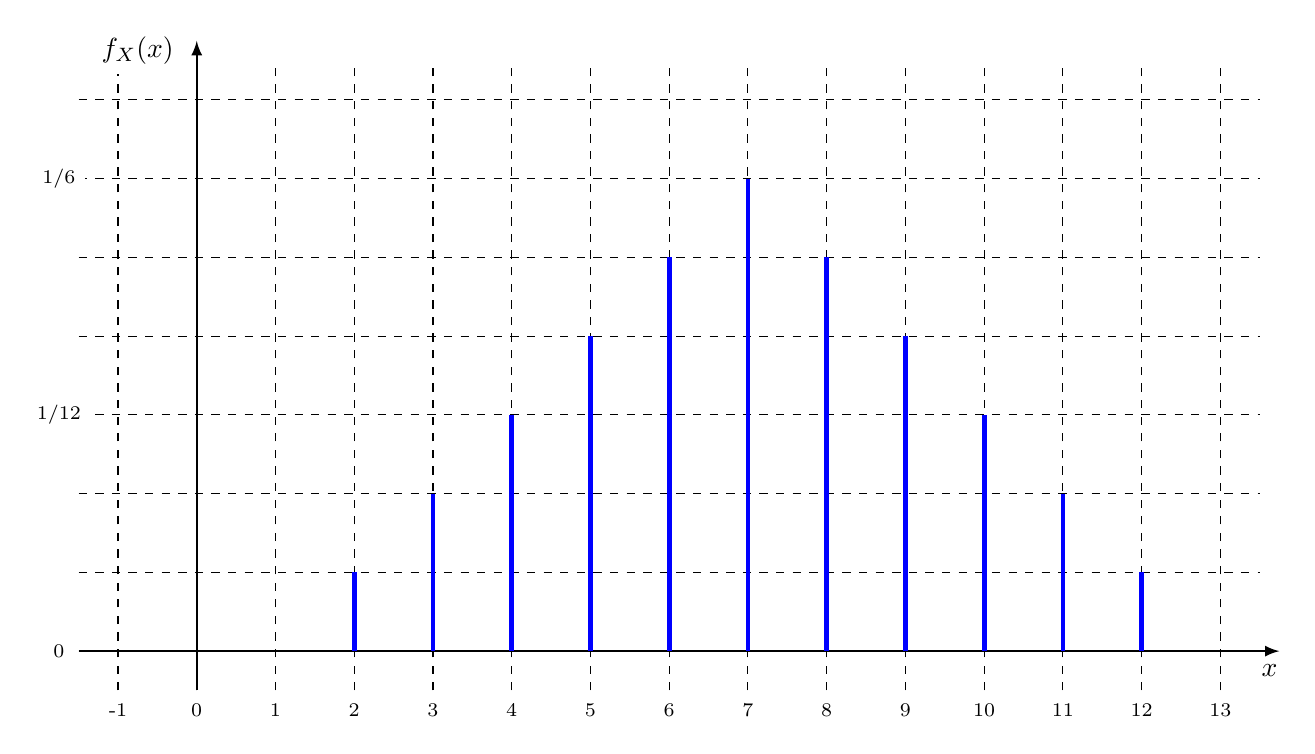
\begin{tikzpicture}
  \draw[-latex,thick] (-1.5,0) -- (13.75,0);
  \node at (13.625,-0.25) {$x$};
  \draw[-latex,thick] (0,-0.5) -- (0,7.75);
  \foreach \x in {-1,...,13}
    \draw[dashed] (\x,-0.5) -- (\x,7.5);
  \foreach \y in {0,...,7}
    \draw[dashed] (-1.5,\y) -- (13.5,\y);
  \node[fill=white] at (-0.75,7.625) {$f_X(x)$};

  \draw[line width=0.6mm,blue] ( 2,0) -- ( 2,1);
  \draw[line width=0.6mm,blue] ( 3,0) -- ( 3,2);
  \draw[line width=0.6mm,blue] ( 4,0) -- ( 4,3);
  \draw[line width=0.6mm,blue] ( 5,0) -- ( 5,4);
  \draw[line width=0.6mm,blue] ( 6,0) -- ( 6,5);
  \draw[line width=0.6mm,blue] ( 7,0) -- ( 7,6);
  \draw[line width=0.6mm,blue] ( 8,0) -- ( 8,5);
  \draw[line width=0.6mm,blue] ( 9,0) -- ( 9,4);
  \draw[line width=0.6mm,blue] (10,0) -- (10,3);
  \draw[line width=0.6mm,blue] (11,0) -- (11,2);
  \draw[line width=0.6mm,blue] (12,0) -- (12,1);
  
  \foreach \x in {-1,...,13}
    \node at (\x,-0.75) {\scriptsize \x};
  \node[fill=white] at (-1.75,0) {\scriptsize 0};
  \node[fill=white] at (-1.75,3) {\scriptsize 1/12};
  \node[fill=white] at (-1.75,6) {\scriptsize 1/6};
\end{tikzpicture}
%%%
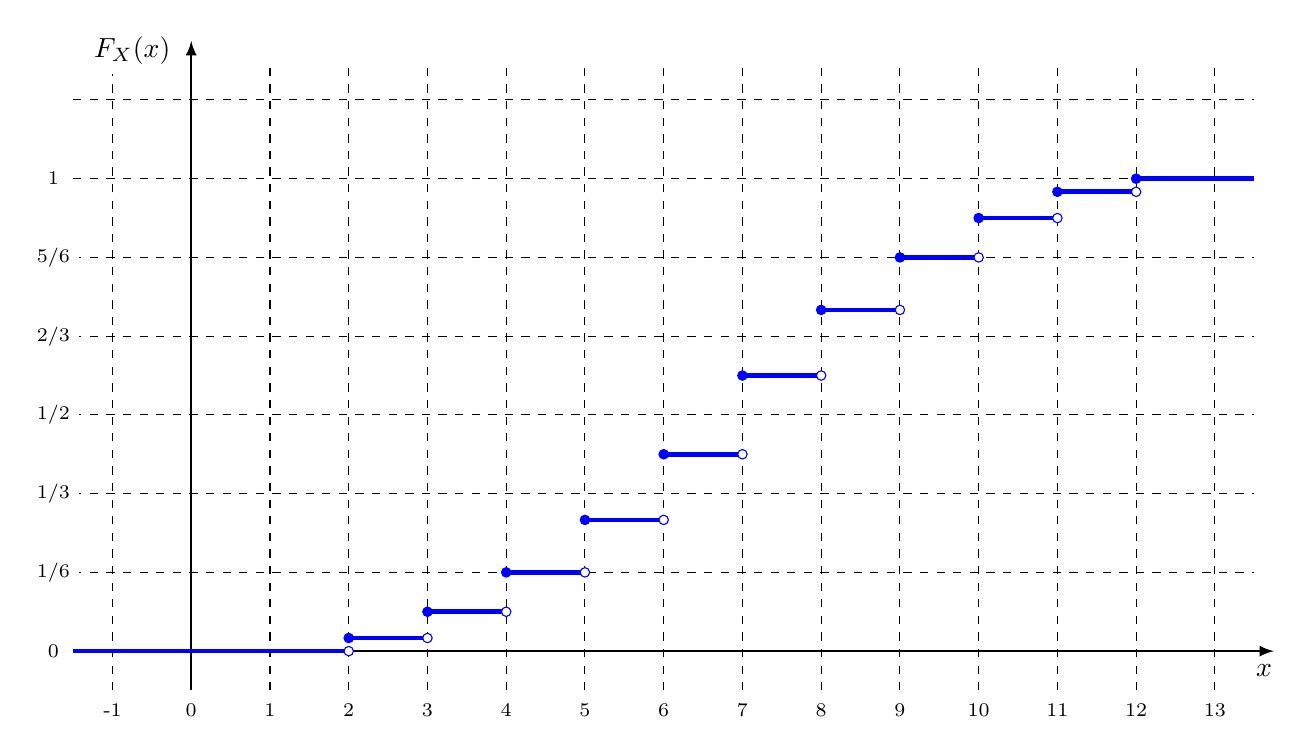
\begin{tikzpicture}
  \draw[-latex,thick] (-1.5,0) -- (13.75,0);
  \node at (13.625,-0.25) {$x$};
  \draw[-latex,thick] (0,-0.5) -- (0,7.75);
  \foreach \x in {-1,...,13}
    \draw[dashed] (\x,-0.5) -- (\x,7.5);
  \foreach \y in {0,...,7}
    \draw[dashed] (-1.5,\y) -- (13.5,\y);
  \node[fill=white] at (-0.75,7.625) {$F_X(x)$};

  \draw[line width=0.6mm,blue] (-1.5,0) -- ( 2,0);
  \draw[blue,fill=white] ( 2,0) circle (0.6mm);
%%%
  \draw[line width=0.6mm,blue] (2,{1/6}) -- ( 3,{1/6});
  \draw[blue,fill=blue]  ( 2,{1/6}) circle (0.6mm);
  \draw[blue,fill=white] ( 3,{1/6}) circle (0.6mm);
%%%
  \draw[line width=0.6mm,blue] (3,{1/2}) -- ( 4,{1/2});
  \draw[blue,fill=blue]  ( 3,{1/2}) circle (0.6mm);
  \draw[blue,fill=white] ( 4,{1/2}) circle (0.6mm);
%%%
  \draw[line width=0.6mm,blue] (4,{1}) -- ( 5,{1});
  \draw[blue,fill=blue]  ( 4,{1}) circle (0.6mm);
  \draw[blue,fill=white] ( 5,{1}) circle (0.6mm);
%%%
  \draw[line width=0.6mm,blue] (5,{5/3}) -- ( 6,{5/3});
  \draw[blue,fill=blue]  ( 5,{5/3}) circle (0.6mm);
  \draw[blue,fill=white] ( 6,{5/3}) circle (0.6mm);
%%%
  \draw[line width=0.6mm,blue] (6,{5/2}) -- ( 7,{5/2});
  \draw[blue,fill=blue]  ( 6,{5/2}) circle (0.6mm);
  \draw[blue,fill=white] ( 7,{5/2}) circle (0.6mm);
%%%
  \draw[line width=0.6mm,blue] (7,{7/2}) -- ( 8,{7/2});
  \draw[blue,fill=blue]  ( 7,{7/2}) circle (0.6mm);
  \draw[blue,fill=white] ( 8,{7/2}) circle (0.6mm);
%%%
  \draw[line width=0.6mm,blue] (8,{13/3}) -- ( 9,{13/3});
  \draw[blue,fill=blue]  ( 8,{13/3}) circle (0.6mm);
  \draw[blue,fill=white] ( 9,{13/3}) circle (0.6mm);
%%%
  \draw[line width=0.6mm,blue] (9,{5}) -- (10,{5});
  \draw[blue,fill=blue]  ( 9,{5}) circle (0.6mm);
  \draw[blue,fill=white] (10,{5}) circle (0.6mm);
%%%
  \draw[line width=0.6mm,blue] (10,{11/2}) -- (11,{11/2});
  \draw[blue,fill=blue]  (10,{11/2}) circle (0.6mm);
  \draw[blue,fill=white] (11,{11/2}) circle (0.6mm);
%%%
  \draw[line width=0.6mm,blue] (11,{35/6}) -- (12,{35/6});
  \draw[blue,fill=blue]  (11,{35/6}) circle (0.6mm);
  \draw[blue,fill=white] (12,{35/6}) circle (0.6mm);
%%%
  \draw[line width=0.6mm,blue] (12,{6}) -- (13.5,{6});
  \draw[blue,fill=blue]  (12,{6}) circle (0.6mm);
%%%
  \foreach \x in {-1,...,13}
    \node at (\x,-0.75) {\scriptsize \x};
  \node[fill=white] at (-1.75,0) {\scriptsize 0};
  \node[fill=white] at (-1.75,1) {\scriptsize 1/6};
  \node[fill=white] at (-1.75,2) {\scriptsize 1/3};
  \node[fill=white] at (-1.75,3) {\scriptsize 1/2};
  \node[fill=white] at (-1.75,4) {\scriptsize 2/3};
  \node[fill=white] at (-1.75,5) {\scriptsize 5/6};
  \node[fill=white] at (-1.75,6) {\scriptsize 1};
%  \draw[line width=0.6mm,blue] ( 3,0) -- ( 3,2);
%  \draw[line width=0.6mm,blue] ( 4,0) -- ( 4,3);
%  \draw[line width=0.6mm,blue] ( 5,0) -- ( 5,4);
%  \draw[line width=0.6mm,blue] ( 6,0) -- ( 6,5);
%  \draw[line width=0.6mm,blue] ( 7,0) -- ( 7,6);
%  \draw[line width=0.6mm,blue] ( 8,0) -- ( 8,5);
%  \draw[line width=0.6mm,blue] ( 9,0) -- ( 9,4);
%  \draw[line width=0.6mm,blue] (10,0) -- (10,3);
%  \draw[line width=0.6mm,blue] (11,0) -- (11,2);
%  \draw[line width=0.6mm,blue] (12,0) -- (12,1);
\end{tikzpicture}
\caption{Probability mass and cumulative distribution functions for the sum of two six-sided dice.}
\label{Fig:probability_sumTwoDiceExample}
\end{center}
\end{figure}


%%%%%%%%%%%%%%%%%%%%%%%%%%%%%%%%%%%%%%%%%%%%%%%%%%%%%%%%%%%%%%%%%%%%%%%%%%%%%%%%%%%%%%%%%%%%%%%
\subsection{Example: Nuclear Reaction Probabilities}

When two particles interact, the outcome of that interaction is inherently random because of the laws of quantum mechanics. Here we will consider the case of a neutron interacting the a fissile nucleus such as $^{235}$U. In this case there are three different types of nuclear reactions that may occur: elastic scattering, radiative capture (n,$\gamma$), and nuclear fission. 

The total likelihood of interaction is governed by the microscopic total cross section $\sigma_t$ (which is a strong function of the neutron kinetic energy, but we will ignore this for the time being). Each individual reaction has a cross section: elastic scattering is $\sigma_s$; radiative capture is $\sigma_\gamma$, and fission is $\sigma_f$. The reaction probabilities are given by the ratio of the reaction cross section divided by the total cross section. For example, the probability of fission $p_f = \sigma_f / \sigma_t$.

Suppose we have $\sigma_t = 4$~b, $\sigma_s = 2.5$~b, $\sigma_c = 0.5$~b, and $\sigma_f = 1$~b. the reaction probabilities are $p_s = \tfrac{5}{8}$, $p_c = \tfrac{1}{8}$, and $p_f = \tfrac{1}{4}$. If we number these as 1 being scattering, 2 being radiative capture, and 3 being nuclear fission, we can compute the probability mass function and cumulative distribution function. The probability mass function is
\begin{align}
  f_X(x) &= \left\{ \begin{array}{r l}
  \frac{5}{8},  & \quad x = 1, \text{elastic scattering} \vspace{0.2cm} \\
  \frac{1}{8},  & \quad x = 2, \text{radiative capture} \vspace{0.2cm} \\
  \frac{1}{4},  & \quad x = 3, \text{nuclear fission} \vspace{0.2cm} \\
  0,            & \quad \text{otherwise} \\ \end{array} \right. ,
\end{align}
and the cumulative distribution function is
\begin{align}
  F_X(x) &= \left\{ \begin{array}{r l}
  0, & \quad x < 1 \vspace{0.2cm} \\
  \frac{5}{8},   & \quad 1  \le x < 2  \vspace{0.2cm} \\ 
  \frac{3}{4},   & \quad 2  \le x < 3  \vspace{0.2cm} \\ 
  1,             & \quad x \ge 3  \vspace{0.2cm} \\ \end{array} \right. .
\end{align}



%%%%%%%%%%%%%%%%%%%%%%%%%%%%%%%%%%%%%%%%%%%%%%%%%%%%%%%%%%%%%%%%%%%%%%%%%%%%%%%%%%%%%%%%%%%%%%%
%%%%%%%%%%%%%%%%%%%%%%%%%%%%%%%%%%%%%%%%%%%%%%%%%%%%%%%%%%%%%%%%%%%%%%%%%%%%%%%%%%%%%%%%%%%%%%%
\section{Continuous Random Variables}

In the previous section, we introduced the concept of random variables for the case that they can take on discrete values. We can also talk about random variables that can take on a continuum of values. The support may be finite or infinite. Examples of continuous random variables are
\begin{itemize}
  \item The time for pump in a nuclear power plant to fail from its installation date;
  \item The distance a photon travels before undergoing an interaction with an electron in a solid;
  \item The kinetic energy of a neutron emitted from fission;
  \item The thickness of a component in given uncertainties in the manufacturing process (dimensional tolerances).
\end{itemize}

In this section, we will introduce the probability density function and the cumulative distribution function for continuous random variables. These concepts are similar, but do differ from the discrete case and warrant separate discussion. We will then give a few examples and discuss common continuous random distributions.

%%%%%%%%%%%%%%%%%%%%%%%%%%%%%%%%%%%%%%%%%%%%%%%%%%%%%%%%%%%%%%%%%%%%%%%%%%%%%%%%%%%%%%%%%%%%%%%
\subsection{Probability Density Function}

The probability density function is the analog of the probability mass function of discrete random variables, but for continuous random variables. The major difference is that the probability density function does not return a probability, but rather a probability density, which is probability per whatever unit the random variable has, e.g., probability per unit length, probability per unit time, etc.

The probability that a random variable $X$ with have a result between $x$ and $x + dx$ is given as
\begin{align}
  f_X(x) dx = P( x \le X \le x + dx ) .
\end{align}
To get a probability, we take the area under the curve of a probability density function:
\begin{align}
  P( a \le X \le b ) = \int_a^b f_X(x) dx .
\end{align}
The probability density function satisfies the normalization property that
\begin{align}
  \int_{-\infty}^\infty f_X(x) dx = 1.
\end{align}
The probability density function satisfies the property that it is never negative:
\begin{align}
  f_X(x) \ge 0.
\end{align}
Since the probability density function is not a probability, it is not restricted to be less than or equal to one. On the contrary, it is often the case that a probability density function has portions that are greater than one, so long as the area under the curve of any region is always less than or equal to one. 

%%%%%%%%%%%%%%%%%%%%%%%%%%%%%%%%%%%%%%%%%%%%%%%%%%%%%%%%%%%%%%%%%%%%%%%%%%%%%%%%%%%%%%%%%%%%%%%
\subsection{Cumulative Distribution Function}

There is also a version of the cumulative distribution function for continuous random variables. Similar to discrete random variables, the cumulative distribution is the probability that a continuous random variable $X$ is at most a value $x$:
\begin{align}
  F_X(x) = P( X \le x ),
\end{align}
which may be obtained from the integral
\begin{align}
  F_X(x) = \int_{-\infty}^x f_X(x') dx' .
\end{align}
The cumulative distribution function is a monotonically increasing function again satisfying:
\begin{align}
  F_X(-\infty) &= 0, \nonumber \\
  F_X(\infty)  &= 1. \nonumber
\end{align}
Because the cumulative distribution function is a continuous function, we can get the corresponding probability density function from
\begin{align}
  f_X(x) = \frac{dF_X}{dx} .
\end{align}


%%%%%%%%%%%%%%%%%%%%%%%%%%%%%%%%%%%%%%%%%%%%%%%%%%%%%%%%%%%%%%%%%%%%%%%%%%%%%%%%%%%%%%%%%%%%%%%
\subsection{Example: Radioactive Decay}

An important application of continuous random variables in nuclear engineering is radioactive decay, which follows an exponential decay law. The probability density function for the exponential decay law is 
\begin{align}
  f_T(t) = \left\{ \begin{array}{r l} 
    \lambda e^{-\lambda t}, & \quad t \ge 0 \\
    0, & \quad \text{otherwise} \\ \end{array} \right. 
\end{align}
where $\lambda$ is the decay constant, which has units of inverse time. We can show that the exponential distribution is indeed normalized:
\begin{align}
  \int_{-\infty}^\infty f_T(t) dt = \int_{-\infty}^0 0 dt + \int_0^{\infty} \lambda e^{-\lambda t} dt = 0 + \lambda \frac{1}{\lambda} = 1 .
\end{align}
If we want to know the probability a radioisotope decays by a certain time, we can calculate the cumulative distribution function:
\begin{align}
  F_T(t) = \int_{-\infty}^t f_T(t') dt' = \int_0^t  \lambda e^{-\lambda t'} dt' = 1 - e^{-\lambda t}, \quad t \ge 0 .
\end{align}
If $t < 0$, the cumulative distribution function is zero.


%%%%%%%%%%%%%%%%%%%%%%%%%%%%%%%%%%%%%%%%%%%%%%%%%%%%%%%%%%%%%%%%%%%%%%%%%%%%%%%%%%%%%%%%%%%%%%%
\subsection{Example: Piecewise-Linear Function}

It is common to represent probability density functions of more complicated functions as piecewise-constant or piecewise-linear functions. An example of this is as follows:
\begin{align}
  f_X(x) = \left\{ \begin{array}{r l} 
    C ( 1 + x ),            & \quad -1 \le x \le 0 \vspace{0.2cm} \\
    C ( 1 - \tfrac{x}{2} ), & \quad  0 \le x \le 2 \vspace{0.2cm} \\
    0, & \quad \text{otherwise} \vspace{0.2cm} \\ \end{array} \right. .
\end{align}
Here $C$ is a normalization constant we need to determine. To find this, we integrate the probability density function from $-\infty$ to $\infty$, set the result equal to 1, and solve for the constant. This proceeds as
\begin{align}
  \int_{-\infty}^\infty f_X(x) &= \int_{-1}^0 C ( 1 + x ) dx + \int_0^2 C ( 1 - \tfrac{x}{2} ) dx = 1 \nonumber \\
  &= \frac{3}{2} C = 1
\end{align}
Therefore, the constant is $C = \tfrac{2}{3}$ and we can rewrite the probability density function as
\begin{align}
  f_X(x) = \left\{ \begin{array}{r l} 
    \tfrac{2}{3} ( 1 + x ),            & \quad -1 \le x \le 0 \vspace{0.2cm} \\
    \tfrac{2}{3} ( 1 - \tfrac{x}{2} ), & \quad  0 < x \le 2 \vspace{0.2cm} \\
    0, & \quad \text{otherwise} \vspace{0.2cm} \\ \end{array} \right. .
\end{align}
This probability density function is plotted in Fig.~\ref{Fig:probability_piecewiseLinearExample}.

\begin{figure}[tb!]
\begin{center}
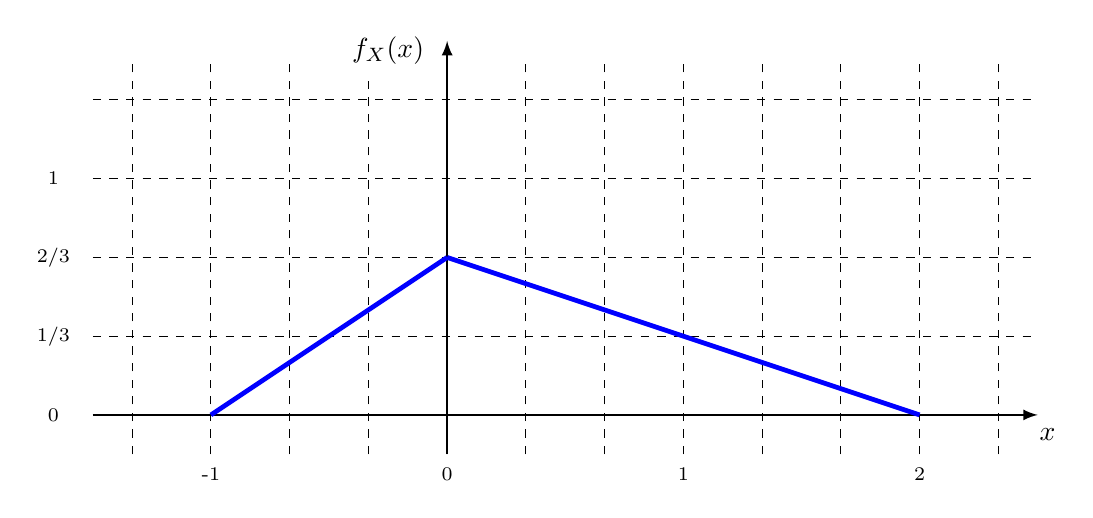
\begin{tikzpicture}
  \draw[-latex,thick] (-4.5,0) -- (7.5,0);
  \node at (7.625,-0.25) {$x$};
  \draw[-latex,thick] (0,-0.5) -- (0,4.75);
  \foreach \x in {-4,...,7}
    \draw[dashed] (\x,-0.5) -- (\x,4.5);
  \foreach \y in {0,...,4}
    \draw[dashed] (-4.5,\y) -- (7.5,\y);
  \node[fill=white] at (-0.75,4.625) {$f_X(x)$};
  
  \draw[line width=0.6mm,blue] (-3,0) -- (0,2);
  \draw[line width=0.6mm,blue] (0,2)  -- (6,0);
  
  \foreach \x in {-1,...,2}
    \node at ({3*\x},-0.75) {\scriptsize \x};
  \node[fill=white] at (-5.0,0) {\scriptsize 0};
  \node[fill=white] at (-5.0,1) {\scriptsize 1/3};
  \node[fill=white] at (-5.0,2) {\scriptsize 2/3};
  \node[fill=white] at (-5.0,3) {\scriptsize 1};
\end{tikzpicture}
%%%
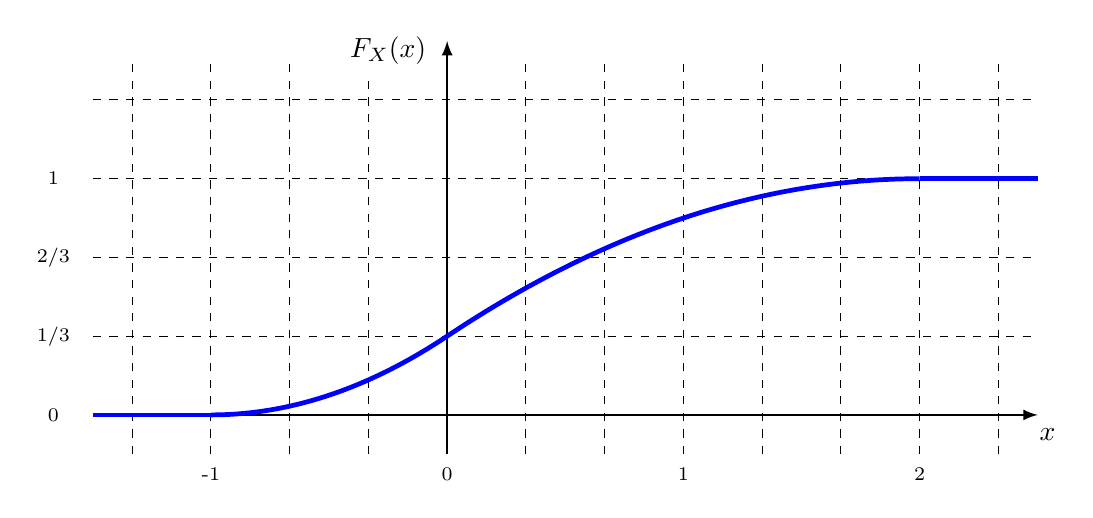
\begin{tikzpicture}
  \draw[-latex,thick] (-4.5,0) -- (7.5,0);
  \node at (7.625,-0.25) {$x$};
  \draw[-latex,thick] (0,-0.5) -- (0,4.75);
  \foreach \x in {-4,...,7}
    \draw[dashed] (\x,-0.5) -- (\x,4.5);
  \foreach \y in {0,...,4}
    \draw[dashed] (-4.5,\y) -- (7.5,\y);
  \node[fill=white] at (-0.75,4.625) {$F_X(x)$};
  
  \draw[line width=0.6mm,blue] (-4.5,0) -- (-3,0);
  \draw[line width=0.6mm,blue] plot[smooth,domain=-1:0] ({3*\x}, {( 1 + 2*\x + \x*\x )});
  \draw[line width=0.6mm,blue] plot[smooth,domain= 0:2] ({3*\x}, {( 1 + 2*\x - 0.5*\x*\x )});
  \draw[line width=0.6mm,blue] (6,3)  -- (7.5,3);
  
  \foreach \x in {-1,...,2}
    \node at ({3*\x},-0.75) {\scriptsize \x};
  \node[fill=white] at (-5.0,0) {\scriptsize 0};
  \node[fill=white] at (-5.0,1) {\scriptsize 1/3};
  \node[fill=white] at (-5.0,2) {\scriptsize 2/3};
  \node[fill=white] at (-5.0,3) {\scriptsize 1};
\end{tikzpicture}
\caption{Probability density and cumulative distribution functions for the piecewise-linear function.}
\label{Fig:probability_piecewiseLinearExample}
\end{center}
\end{figure}

To obtain the cumulative distribution function, we consider each range. For the range with $x < -1$, the cumulative distribution function is zero. For the range between $-1 \le x \le 0$, we evaluate
\begin{align}
  F_X(x) &= \int_{-1}^x \tfrac{2}{3} ( 1 + x' ) dx' = \frac{1}{3} ( 1 + 2 x + x^2 ) .
\end{align}
For the range between $0 < x \le 2$, we must integrate the previous region up to 0 and the following region up to $x$:
\begin{align}
  F_X(x) &= \int_{-1}^0 \tfrac{2}{3} ( 1 + x' ) dx' + \int_{-1}^x \tfrac{2}{3} ( 1 - \tfrac{x'}{2} ) dx' \nonumber \\
  &= \tfrac{1}{3} ( 1 + 2 x - \tfrac{1}{2} x^2 ) .
\end{align}
We can verify that $F_X(2) = 1$, and since the probability density function is zero for $x > 2$, the cumulative density function will remain one. Pulling this together we have
\begin{align}
  F_X(x) = \left\{ \begin{array}{r l}
    0, & \quad x < 2  \vspace{0.2cm} \\
    \frac{1}{3} ( 1 + 2 x + x^2 ),            & \quad -1 \le x \le 0 \vspace{0.2cm} \\
    \tfrac{1}{3} ( 1 + 2 x - \tfrac{1}{2} x^2 ), & \quad  0 < x \le 2 \vspace{0.2cm} \\
    1, & \quad x > 2 \vspace{0.2cm} \\ \end{array} \right. .
\end{align}
This is also plotted in Fig.~\ref{Fig:probability_piecewiseLinearExample}.


%%%%%%%%%%%%%%%%%%%%%%%%%%%%%%%%%%%%%%%%%%%%%%%%%%%%%%%%%%%%%%%%%%%%%%%%%%%%%%%%%%%%%%%%%%%%%%%
%%%%%%%%%%%%%%%%%%%%%%%%%%%%%%%%%%%%%%%%%%%%%%%%%%%%%%%%%%%%%%%%%%%%%%%%%%%%%%%%%%%%%%%%%%%%%%%
\section{Multivariate Distributions}

In the previous sections we introduced discrete and continuous random variables in the context of a single random variable. It is common to have multiple random variables simultaneous that may or may not be independent. Most of the following discussion will focus on the case of two random variables, but the concepts are generalizable to any number.

%%%%%%%%%%%%%%%%%%%%%%%%%%%%%%%%%%%%%%%%%%%%%%%%%%%%%%%%%%%%%%%%%%%%%%%%%%%%%%%%%%%%%%%%%%%%%%%
\subsection{Probability Mass/Density Functions}

We can generalize the probability mass function and probability density function to multiple variables in a relatively straightforward manner. The joint probability mass function for two random variables $X$ and $Y$ describes the joint probability that $X = x$ and $Y = y$. This is
\begin{align}
  f_{X,Y}(x,y) = P( X = x, Y = y ) .
\end{align}
If we are given the joint probability mass function want to compute the probability mass function of a single random variable $X$ or $Y$, we sum over the other variable(s):
\begin{subequations}
\begin{align}
  f_X(x) &= \sum_y f_{X,Y}(x,y), \\*
  f_Y(x) &= \sum_x f_{X,Y}(x,y).
\end{align}
\end{subequations}
If we have more than two, we sum over all the variables that we do not want information about. The single variable probability mass functions derived from a joint probability mass function are called the marginal probability mass function.

The probability density function for the two variable case is defined so that the probability that random variable $X$ is between $x$ and $x + dx$ and $Y$ is between $y$ and $y + dy$ is
\begin{align}
  f_{X,Y}(x,y)dxdy = P( x \le X \le x + dx, y \le Y \le y + dy ) .
\end{align}
Similar to the single variable case, the units of the probability density function are probability per the units of random variable $X$ per the units of random variable $Y$. In a similar manner to the discrete case, we can compute the marginal probability density functions in $X$ and $Y$ alone by integrating out the variables that are not of interest:
\begin{subequations}
\begin{align}
  f_X(x) &= \int_{-\infty}^\infty f_{X,Y}(x,y) dy, \\*
  f_Y(x) &= \int_{-\infty}^\infty f_{X,Y}(x,y) dx.
\end{align}
\end{subequations}

The final point to bring up in this section is the case where random variables $X$ and $Y$ are independent. In this case we may write the joint probability mass or density function as the product of the marginals:
\begin{align}
  f_{X,Y}(x,y) = f_X(x) f_Y(y), \quad \text{only if $X$ and $Y$ are independent.}
\end{align}

%%%%%%%%%%%%%%%%%%%%%%%%%%%%%%%%%%%%%%%%%%%%%%%%%%%%%%%%%%%%%%%%%%%%%%%%%%%%%%%%%%%%%%%%%%%%%%%
\subsection{Cumulative Distribution Functions}

It may not be surprising that we can also generalize the cumulative distribution functions to multiple variables. In both cases this states that random variables $X$ and $Y$ are simultaneously at most $x$ and $y$ respectively. For the discrete random variable case, the cumulative distribution function for random variables $X$ and $Y$ is
\begin{align}
  F_{X,Y}(x,y) = \sum_{x_i < x} \sum_{y_i < y} f_{X,Y}(x_i,y_i) = P( X \le x, Y \le Y ).
\end{align}
The cumulative distribution for the continuous case is
\begin{align}
  F_{X,Y}(x,y) = \int_{-\infty}^y \int_{-\infty}^x f_{X,Y}(x',y') dx' dy' = P( X \le x, Y \le Y ).
\end{align}


%%%%%%%%%%%%%%%%%%%%%%%%%%%%%%%%%%%%%%%%%%%%%%%%%%%%%%%%%%%%%%%%%%%%%%%%%%%%%%%%%%%%%%%%%%%%%%%
\subsection{Conditional Distribution Functions}

Earlier on we discussed the idea of conditional probability, which is the idea that the probability of a particular event outcome is influenced by the outcome of a different, but related random event. The notion of conditional probability also can be applied in the context of probability mass/density functions and their cumulative distribution function counterparts. 

The conditional probability mass function for a discrete random variable is the probability random variable $X = x$ given that we know another random variable $Y = y$. This is written as
\begin{align}
  f_{X|Y}(x,y) = P( X = x | Y = y ) .
\end{align}
The cumulative distribution function is the probability that $X \le x$ given that $Y = y$ and is computed by as follows:
\begin{align}
  F_{X|Y}(x,y) = \sum_{x_i < x} f_{X|Y}(x_i) = P( X \le x | Y = y ) .
\end{align}

The conditional probability density function is defined similarly as before. The probability that random variable $X$ is between $x$ and $x + dx$ given that random variable $Y = y$ is
\begin{align}
  f_{X|Y}(x,y) dx = P( X = x | Y = y ) ,
\end{align}
and the cumulative distribution function is
\begin{align}
  F_{X|Y}(x,y) = \int_{-\infty}^x f_{X|Y}(x') dx' = P( X \le x | Y = y ) .
\end{align}

We can relate the conditional probability mass or density functions to the joint mass or density functions for either the discrete or continuous case:
\begin{align}
  f_{X,Y}(x,y) = f_{Y|X}(x,y) f_Y(x) = f_{X|Y}(x,y) f_Y(y) .
\end{align}


%%%%%%%%%%%%%%%%%%%%%%%%%%%%%%%%%%%%%%%%%%%%%%%%%%%%%%%%%%%%%%%%%%%%%%%%%%%%%%%%%%%%%%%%%%%%%%%
\subsection{Example: Discrete Binary Distribution}

Suppose we have two random variables $X$ and $Y$ that both take on the value of zero or one. The probability mass function is given by the function
\begin{align}
  f_{X,Y}(x,y) = C \frac{ 1 + 3x }{ 1 + xy }, \quad x \in \left\{ 0, 1 \right\}, \quad y \in \left\{ 0, 1 \right\} .
\end{align}
We wish to find the marginal probability mass functions.

First, we normalize the distribution function by taking
\begin{align}
  \sum_{x=0}^1 \sum_{y=0}^1 C \frac{ 1 + 2x }{ 1 + y } &= 
  C \left( \frac{ 1 + 3(0) }{ 1 + (0)(0) } + \frac{ 1 + 3(0) }{ 1 + (0)(1) } + \frac{ 1 + 3(1) }{ 1 + (1)(0) } + \frac{ 1 + 3(1) }{ 1 + (1)(1) } \right) \nonumber \\
  &= C \left( 1 + 1 + 4 + 2 \right) = 8 C = 1 .
\end{align}
Therefore $C = \tfrac{1}{8}$. Rewriting the probability mass function gives
\begin{align}
  f_{X,Y}(x,y) = \frac{ 1 + 3x }{ 8 ( 1 + xy ) }, \quad x \in \left\{ 0, 1 \right\}, \quad y \in \left\{ 0, 1 \right\} .
\end{align}

To find the marginal probability mass functions in $x$ and $y$, we sum over $y$ and $x$ respectively. The marginal probability mass function in $x$ is
\begin{align}
  f_X(x) = \sum_{y=0}^1 f_{X,Y}(x,y) &= \frac{ 1 + 3x }{ 8 ( 1 + 0 ) } + \frac{ 1 + 2x }{ 8 ( 1 + x ) } \nonumber \\
  &=  \frac{ ( 1 + 3x ) ( 1 + x ) }{ 8 ( 1 + x ) } + \frac{ 1 + 3x }{ 8 ( 1 + x ) } \nonumber \\
  &=  \frac{ 3x^2 + 7x + 2 }{ 8 ( 1 + x ) } .
\end{align}
The marginal probability mass function in $y$ is
\begin{align}
  f_Y(y) = \sum_{x=0}^1 f_{X,Y}(x,y) &= \frac{ 1 }{ 8 ( 1 + 0 ) } + \frac{ 1 + 2 }{ 8 ( 1 + y ) } \nonumber \\
  &=  \frac{1}{8} \left( 1 + \frac{3}{1+y} \right) \nonumber \\
  &=  \frac{ 4 + y }{ 8 ( 1 + y ) } .
\end{align}

%%%%%%%%%%%%%%%%%%%%%%%%%%%%%%%%%%%%%%%%%%%%%%%%%%%%%%%%%%%%%%%%%%%%%%%%%%%%%%%%%%%%%%%%%%%%%%%
%%%%%%%%%%%%%%%%%%%%%%%%%%%%%%%%%%%%%%%%%%%%%%%%%%%%%%%%%%%%%%%%%%%%%%%%%%%%%%%%%%%%%%%%%%%%%%%
\section{Random Variable Operators}

In this chapter we will discuss the common operators used upon random variables, which are used to extract information about a random variable and its distribution. Here we will cover expectation (the mean value), variance (square of the standard deviation), and covariance (related to correlation).

%%%%%%%%%%%%%%%%%%%%%%%%%%%%%%%%%%%%%%%%%%%%%%%%%%%%%%%%%%%%%%%%%%%%%%%%%%%%%%%%%%%%%%%%%%%%%%%
\subsection{Expectation}

The most important and commonly used operator for random variables is the expectation operator $E(\cdot)$. The expectation operator is often used in the definitions of other operators. The simplest form is to take the expectation of a random variable $E(X)$. The expectation of the discrete and continuous random variables are, respectively,
\begin{subequations}
\begin{align}
  E(X) &= \sum_x x f_X(x), \\
  E(X) &= \int_{-\infty}^\infty x f_X(x) dx .
\end{align}
\end{subequations}
The expectation operator on a random variable produces a number that corresponds to its mean value and we therefore often colloquially call $E(X)$ as the average of random variable $X$. The mean describes the central tendency of the distribution, i.e., where is the probability of the distribution centered about. The concept is similar to the ``center of mass'' from physics.

An important point is that expectation does not necessarily mean the most probable value---although this is sometimes the case, it is often that it does not. For example, let us consider the simple example of a fair coin where we assign heads a value of 1 and tails a value of 0. Since the coin is fair, we have an equal probability of getting heads or tails. The expectation in this case is
\begin{align}
  E(X) = \sum_x x f_X(x) = (0) ( \tfrac{1}{2} ) + (1) ( \tfrac{1}{2} ) = \tfrac{1}{2} . \nonumber
\end{align}
The expectation or mean value is $\tfrac{1}{2}$, which does not correspond to either heads or tails. The takeaway again is that expectation measures centrality of a distribution and not maximal likeliness.

The expectation operator is a linear operator and satisfies the following properties:
\begin{align}
  E(c) &= c, \\*
  E(aX) &= aE(X), \\*
  E(X + Y) &= E(X) + E(Y) .
\end{align}
Here $a$ and $c$ are non-random constants.

Additionally, the result of the expectation operator is related to the sample mean. If we collect $N$ samples $x_i$ from random variable $X$, we can estimate the mean using the sample mean
\begin{align}
  E(X) \approx \overline{x} = \frac{1}{N} \sum_{i=1}^N x_i .
\end{align}
The approximation becomes exact in the limit as $N \rightarrow \infty$, provided that the expectation exists. There are certain pathological cases (see the Cauchy distribution) where there is no mean value. In this case, the sample mean will never converge to any value.

We can extend the expactation operator to take what we call moments of a random variable. For example, the second moment is
\begin{subequations}
\begin{align}
  E(X^2) &= \sum_x x^2 f_X(x), \\*
  E(X^2) &= \int_{-\infty}^\infty x^2 f_X(x) dx ,
\end{align}
\end{subequations}
for discrete and continuous random variables respectively. The second moment is useful in defining the variance operator, which is covered in the next section.

We can further generalize the expectation to consider any function of a random variable. We define
\begin{subequations}
\begin{align}
  E(g(X)) &= \sum_x g(x) f_X(x), \\*
  E(g(X)) &= \int_{-\infty}^\infty g(x) f_X(x) dx ,
\end{align}
\end{subequations}
again for the respective discrete and continuous cases.

We can generalize the concept to multiple variables by stating that the expectation operator always returns a number. If we have a bivariate joint random distribution for $X$ and $Y$, the expectation of the random variable $X$ is
\begin{subequations}
\begin{align}
  E(X) &= \sum_x \sum_y x f_{X,Y}(x,y) = \sum_x x f_X(x), \\*
  E(X) &= \int_{-\infty}^\infty \int_{-\infty}^\infty x f_{X,Y}(x,y) dy dx = \int_{-\infty}^\infty x f_X(x) dx .
\end{align}
\end{subequations}
Furthermore, we take the expectation with any function of random variables $g(X,Y)$ using
\begin{subequations}
\begin{align}
  E(g(X,Y)) &= \sum_x \sum_y g(x,y) f_{X,Y}(x,y), \\*
  E(g(X,Y)) &= \int_{-\infty}^\infty \int_{-\infty}^\infty g(x,y) f_{X,Y}(x,y) dy dx .
\end{align}
\end{subequations}
We can get an estimate from the sample mean for this case if we have $N$ samples of $x_i$ and $y_i$ using
\begin{align}
  E(g(X,Y)) \approx \frac{1}{N} \sum_{i=1}^{N} g(x_i,y_i) ,
\end{align}
where the approximation becomes exact in the limit as $N \rightarrow \infty$ provided the expectation exists.

A final important property is independence related to the term $E(XY)$. If $X$ and $Y$ are independent, then we can show that $E(XY) = E(X)E(Y)$. This is
\begin{align}
  E(XY) &= \int_{-\infty}^\infty \int_{-\infty}^\infty xy f_{X,Y}(x,y) \nonumber \\*
  &= \int_{-\infty}^\infty \int_{-\infty}^\infty xy f_X(x) f_Y(y) \nonumber \\*
  &= \left(  \int_{-\infty}^\infty x f_X(x) dx \right) \left( \int_{-\infty}^\infty y f_Y(y) dy \right) \nonumber \\*
  &= E(X)E(Y), \quad \text{ if $X$ and $Y$ are independent.}
\end{align}

%%%%%%%%%%%%%%%%%%%%%%%%%%%%%%%%%%%%%%%%%%%%%%%%%%%%%%%%%%%%%%%%%%%%%%%%%%%%%%%%%%%%%%%%%%%%%%%
\subsection{Variance and Standard Deviation}

The variance is the second most commonly encountered operator for random variables. The variance operator is defined as
\begin{align}
  \var ( X ) = E( (X - E(X))^2 ) .
\end{align}
We can expand this out into a more convenient form for calculations:
\begin{align}
  \var ( X ) &= E( X^2 - 2 X E(X) + E(X)^2 ) \nonumber \\*
  &= E(X^2) - 2 E( X E(X) ) + E( E(X)^2 ) \nonumber \\*
  &= E(X^2) - 2 E(X) E(X) + E(X)^2 \nonumber \\*
  &= E(X^2) - E(X)^2 .
\end{align}
Using the variance we can compute the standard deviation
\begin{align}
  \sigma = \sqrt{ \var(X) } .
\end{align}
The standard deviation is a measure of how much the distribution deviates from its mean and can be thought of as how ``spread out'' the probability is. The variance is a strictly positive quantity such that the larger the variance, the more dispersed a the probability of a distribution is relative to its mean.

The variance operator is nonlinear because of the squared term and does not satisfy the linearity properties. However, we can derive another relationship. Suppose we have independent random variables $X$ and $Y$. We then can calculate
\begin{align}
  \var ( aX + bY ) &= E( ( aX + bY )^2 ) - E( aX + bY )^2 \nonumber \\*
  &= E( a^2 X^2 + 2abXY + b^2 Y^2 ) - E( aX + bY ) E( aX + bY ) \nonumber \\*
  &= a^2 E(X^2) + 2ab E(XY) + b^2 E(Y^2) \nonumber \\* &\quad- \left[ aE(X) + bE(Y) \right] \left[ aE(X) + bE(Y) \right] \nonumber \\*
  &= a^2 E(X^2) + 2ab E(X) E(Y) + b^2 E(Y^2) \nonumber \\* &\quad - a^2 E(X)^2 - b^2 E(X)^2 - 2ab E(X) E(Y) \nonumber \\*
  &= a^2 \left[ E(X^2) - E(X)^2 \right] + b^2  \left[ E(Y^2) - E(Y)^2 \right] \nonumber \\*
  &= a^2 \var(X) + b^2 \var(Y) .
\end{align}


%%%%%%%%%%%%%%%%%%%%%%%%%%%%%%%%%%%%%%%%%%%%%%%%%%%%%%%%%%%%%%%%%%%%%%%%%%%%%%%%%%%%%%%%%%%%%%%
\subsection{Covariance and Correlation}

We can also define the covariance between two random variables $X$ and $Y$. The covariance measures how much two random variables change with respect to one another about their respective means. It has the definition of
\begin{align}
  \cov (X,Y) = E[ (X - E(X) ) ( Y - E(Y) ) ] .
\end{align}
This can be expanded out to give the more convenient form for calculation of
\begin{align}
  \cov (X,Y) = E(XY) - E(X) E(Y) .
\end{align}
From the definition, we can see that the covariance of $X$ with itself is simply the variance,
\begin{align}
  \cov (X,X) = E[ (X - E(X) ) ( X - E(X) ) ] = \var(X) .
\end{align}
The covariance is also symmetric:
\begin{align}
  \cov (X,Y) = \cov (Y,X)
\end{align}

If we have multiple random variables, we can define a covariance matrix that contains information about how each random variable varies with respect to the others
\begin{align}
  \boldsymbol\Sigma &=
  \left[ \begin{array}{c c c c}
  \var(X_1)     & \cov(X_1,X_2) & \cdots & \cov(X_1,X_N) \\
  \cov(X_2,X_1) & \var(X_2)     & \cdots & \cov(X_2,X_N) \\
  \vdots        & \vdots        & \ddots & \vdots        \\
  \cov(X_N,X_1) & \cov(X_N,X_2) & \cdots & \var(X_N)     \\ \end{array} \right] .
\end{align}
This covariance matrix is useful when we discuss the propagation of uncertainties.

Unlike the variance, the covariance may be either positive, zero, or negative. To get an interpretation, let us introduce the Pearson correlation coefficient
\begin{align}
  \rho(X,Y) = \frac{ \cov(X,Y) }{ \sqrt{ \var(X) } \sqrt{ \var(Y) } } .
\end{align}
This is the covariance of random variables $X$ and $Y$ divided by the product of their standard deviations. The Pearson correlation coefficient is a scaled covariance that ranges from $-1$ to $1$ and measures linear dependence. Positive correlation implies that if we take a sample of random variables $X$ and $Y$ and if our sample $x$ is high (or low) with respect to its mean, then a corresponding sampled value $y$ will also be high (or low) with respect to its mean. Likewise, if the correlation is negative a low sample of $x$ tends to mean a high sample of $y$.

If the correlation coefficient is zero, then the two random variables are said to be uncorrelated or linearly independent. A common misconception is that a zero correlation or linear independence implies that two random variables are actually independent. The correlation coefficient only measures the linear component of the dependency between two random variables. If, for example, two random variables are only dependent in a purely quadratic nature, the correlation would be zero even though the two random variables are statistically dependent upon each other.



%%%%%%%%%%%%%%%%%%%%%%%%%%%%%%%%%%%%%%%%%%%%%%%%%%%%%%%%%%%%%%%%%%%%%%%%%%%%%%%%%%%%%%%%%%%%%%%
%%%%%%%%%%%%%%%%%%%%%%%%%%%%%%%%%%%%%%%%%%%%%%%%%%%%%%%%%%%%%%%%%%%%%%%%%%%%%%%%%%%%%%%%%%%%%%%
\section{Discrete Distributions}

In this section, we will discuss several common distributions for discrete random variables that are commonly encountered in science and engineering applications.

%%%%%%%%%%%%%%%%%%%%%%%%%%%%%%%%%%%%%%%%%%%%%%%%%%%%%%%%%%%%%%%%%%%%%%%%%%%%%%%%%%%%%%%%%%%%%%%
\subsection{Bernoulli Distribution}

The simplest type of discrete random variable is a Bernoulli distribution. The distribution describes a ``coin flip''. We have a success with probability $p$ that we assign a value of 1, and a failure with probability $1 - p$ that we assign a value of 0. This has the probability mass function of
\begin{align}
  f_X(x) = \left\{ \begin{array}{r l}
  1 - p, & \quad x = 0 \vspace{0.2cm} \\
  p,     & \quad x = 1 \vspace{0.2cm} \\
  0,     & \quad \text{otherwise} \\ \end{array} \right. .
\end{align}
The cumulative distribution function is
\begin{align}
  F_X(x) = \left\{ \begin{array}{r l}
  0      & \quad x < 0 \vspace{0.2cm} \\
  1 - p, & \quad 0 \le x < 1 \vspace{0.2cm} \\
  1,     & \quad x \ge 1 \vspace{0.2cm}  \\ \end{array} \right. .
\end{align}

%%%%%%%%%%%%%%%%%%%%%%%%%%%%%%%%%%%%%%%%%%%%%%%%%%%%%%%%%%%%%%%%%%%%%%%%%%%%%%%%%%%%%%%%%%%%%%%
\subsection{Discrete Uniform Distribution}

Another common distribution is the discrete uniform distribution, which represents the $n$-sided die where each face is equiprobable. Let us enumerate the faces $x = 1, 2, \ldots, n$. The probability mass function is
\begin{align}
  f_X(x) = \left\{ \begin{array}{r l}
  \frac{1}{n}, & \quad x = 1, 2, \ldots, n \vspace{0.2cm} \\
  0,           & \quad \text{otherwise} \\ \end{array} \right. .
\end{align}
The cumulative distribution function is
\begin{align}
  F_X(x) = \left\{ \begin{array}{r l}
  0            & \quad x < 0 \vspace{0.2cm} \\
  \frac{1}{n}, & \quad 0 \le x < 1 \vspace{0.2cm} \\
  \frac{2}{n}, & \quad 1 \le x < 2 \vspace{0.2cm} \\
  \vdots & \\
  \frac{n-1}{n}, & \quad n-1 \le x < n \vspace{0.2cm} \\
  1,     & \quad x \ge n \vspace{0.2cm}  \\ \end{array} \right. .
\end{align}

%%%%%%%%%%%%%%%%%%%%%%%%%%%%%%%%%%%%%%%%%%%%%%%%%%%%%%%%%%%%%%%%%%%%%%%%%%%%%%%%%%%%%%%%%%%%%%%
\subsection{Binomial Distribution}

The binomial distribution describes the number of successful independent trials $n$ of a Bernoulli distribution with probability of success $p$. The probability mass function is
\begin{align}
  f_X(x) = \binom{n}{x} p^x ( 1 - p )^{n-x} , \quad x = 0, \ldots, n 
\end{align}
and zero otherwise. The binomial coefficient may be written in terms of the factorial:
\begin{align}
  \binom{n}{x} = \frac{ n! }{ x! ( n - x )! } 
\end{align}
The binomial coefficient gives the number of unique combinations of $x$ members from a set of $n$ elements. Unfortunately, the cumulative distribution function does not have a form in terms of standard functions and is simply:
\begin{align}
  F_X(x) = \sum_{k=1}^x \binom{n}{k} p^k ( 1 - p )^{n-k} .
\end{align}


%%%%%%%%%%%%%%%%%%%%%%%%%%%%%%%%%%%%%%%%%%%%%%%%%%%%%%%%%%%%%%%%%%%%%%%%%%%%%%%%%%%%%%%%%%%%%%%
\subsection{Example: Determining Number of Experimental Trials}

Suppose we are designing a high-energy density physics experiment that requires collecting data from a laser facility. To collect enough data, we need to ensure we have at least 10 successful shots on the laser facility. We know from historical data of the facility that the success rate of any individual shot is 90\%. We desire a probability of 95\% of having at least 10 successful shots. As part of planning, we need to allocate resources to have a number of shots that gives us this level of confidence that we will meet our objective. Because we have limited resources to purchase time at the laser facility, we want to have as few shots as possible to achieve our desired confidence level.

The appropriate distribution for analyzing this problem is the binomial distribution with $p = 0.9$. To get the number, we know we need at least 10 shots total, so let's start by finding the probability that all 10 shots are successful:
\begin{align}
  P(X \ge 10 ; n = 10) &= f_X(10) \nonumber \\
  &= \binom{10}{10} 0.9^{10} ( 1 - 0.9 )^{10-10} \nonumber \\
  &= \frac{ 10! }{ 10! \times 0! } \times 0.9^{10} \times 0.1^0 = 0.349 . \nonumber
\end{align}
Clearly, just scheduling ten shots would be quite risky and is well below our desired confidence level.

Let's try 11 shots. The probability of having at least 10 successful shots out of 11 is
\begin{align}
  P(X \ge 10 ; n = 11) 
              &= P(X = 10) + P(X = 11) \nonumber \\
              &= f_X(10) + f_X(11) \nonumber \\
              &= \binom{11}{10} 0.9^{10} ( 1 - 0.9 )^{11-10} + \binom{11}{11} 0.9^11 ( 1 - 0.9 )^{11-11} \nonumber \\
              &= 0.3835  +  0.3138 =   0.6974 .
\end{align}
Clearly doing 11 shots improves our chances significantly, but this is still well below our desired confidence level. Let's try 12:
\begin{align}
  P(X \ge 10 ; n = 12 ) &= P(X = 10) + P(X = 11) + P(X = 12) \nonumber \\
                        &= f_X(10) + f_X(11) + f_X(12) \nonumber \\
                        &= 0.2301 + 0.3766 + 0.2824 =  0.8891 .
\end{align}
Getting better, but not quite there yet. Let's schedule a lucky 13 shots:
\begin{align}
  P(X \ge 10 ; n = 13) 
    &= P(X = 10) + P(X = 11) + P(X = 12) + P(X = 13) \nonumber \\
    &= f_X(10) + f_X(11) + f_X(12) + f_X(13) \nonumber \\
    &= 0.0997 + 0.2448 + 0.3672  + 0.2542    =  0.9658  .
\end{align}
Therefore 13 shots achieves our stated objective of having a confidence of at least 95\% of having at least 10 successes.


%%%%%%%%%%%%%%%%%%%%%%%%%%%%%%%%%%%%%%%%%%%%%%%%%%%%%%%%%%%%%%%%%%%%%%%%%%%%%%%%%%%%%%%%%%%%%%%
\subsection{Geometric Distribution}

The geometric distribution can be used to describe the number of successes $x$ before a failure if the failure probability is $p$. For example, we can use the distribution to model the case where we wish to know the number of times a piece of equipment with failure probability $p$ will operate before requiring maintenance. The probability mass function for the geometric distribution is
\begin{align}
  f_X(x) = p ( 1 - p )^x, \quad x \ge 0,
\end{align}
and zero otherwise. The probability mass function gives the exact number of successes before failure. The cumulative distribution function is
\begin{align}
  F_X(x) = 1 - ( 1 - p )^{x+1}, \quad x \ge 0 . 
\end{align}
This is we will have at most $x$ successes before failure. Note that unlike the other distributions we have encountered, the geometric distribution has an infinite support. In other words, when we use the geometric distribution we do not restrict the number of successes that can occur before a failure.

%%%%%%%%%%%%%%%%%%%%%%%%%%%%%%%%%%%%%%%%%%%%%%%%%%%%%%%%%%%%%%%%%%%%%%%%%%%%%%%%%%%%%%%%%%%%%%%
\subsection{Example: Machine Failure Probability}

Suppose the failure probability for a piece of equipment is 0.1\%. If the machine is used everyday, we wish to know the probability that the machine will operator for at least a year, which we take to have 365 days. We let random variable $X$ be the number of days the machine operates successfully before failure. We have
\begin{align}
  P( X \ge 365 ) &= 1 - P( X \le 364 ) \nonumber \\
  &= 1 - F_X(364) \nonumber \\
  &= 1 - \left[ 1 - ( 1 - 0.001 )^{364+1} \right] = 0.999^{365} = 0.694 .
\end{align}


%%%%%%%%%%%%%%%%%%%%%%%%%%%%%%%%%%%%%%%%%%%%%%%%%%%%%%%%%%%%%%%%%%%%%%%%%%%%%%%%%%%%%%%%%%%%%%%
\subsection{Poisson Distribution}

The Poisson distribution can be used to describe the number of radioactive decays during a time $t$ if the sample has a decay constant $\lambda$, which is the expected number of counts per unit time. The probability mass function of the Poisson distribution is
\begin{align}
  f_X(x) = \frac{(\lambda t)^x}{x!} e^{-\lambda t}, \quad x \ge 0,
\end{align}
and zero otherwise. Unfortunately, like the binomial distribution, the Poisson distribution does not have a cumulative distribution function in a closed form.

%%%%%%%%%%%%%%%%%%%%%%%%%%%%%%%%%%%%%%%%%%%%%%%%%%%%%%%%%%%%%%%%%%%%%%%%%%%%%%%%%%%%%%%%%%%%%%%
\subsection{Example: Detecting Radioactive Contamination}

Suppose we have soil that we suspect may be contaminated with a radioactive isotope that does not occur in the environment naturally. The minimum activity of concern is 1~$\mu$Bq/g = $10^{-6}$. If we take a 10~g sample and count the radioactivity for 48 hours and get no counts indicating the specific radioisotope, what is the probability that we got no counts by chance alone assuming we have perfect detection equipment? 

To find this we use the Poisson distribution at $x = 0$. The total activity of the 10~g sample that would be of minimum concern is $10^{-5}$~Bq. We therefore have
\begin{align}
  f_X(0) = \frac{( 1.0\times10^{-6} \times 10 \times 3600 \times 48)^0}{0!} e^{-( 1.0\times10^{-6} \times 10 \times 3600 \times 48)} = 0.178.
\end{align}
This says that even counting for two entire days, we have an 17.8\% chance that a sample with 1~$\mu$Bq/g of activity did not emit any decays and our test would produce a false negative. Since this probability is still rather high, it would be advisable to count for a longer period of time or, if practical, to take a larger sample to establish or rule out contamination. 



%%%%%%%%%%%%%%%%%%%%%%%%%%%%%%%%%%%%%%%%%%%%%%%%%%%%%%%%%%%%%%%%%%%%%%%%%%%%%%%%%%%%%%%%%%%%%%%
%%%%%%%%%%%%%%%%%%%%%%%%%%%%%%%%%%%%%%%%%%%%%%%%%%%%%%%%%%%%%%%%%%%%%%%%%%%%%%%%%%%%%%%%%%%%%%%
\section{Continuous Distributions}

%%%%%%%%%%%%%%%%%%%%%%%%%%%%%%%%%%%%%%%%%%%%%%%%%%%%%%%%%%%%%%%%%%%%%%%%%%%%%%%%%%%%%%%%%%%%%%%
\subsection{Uniform Distribution}

The simplest of the continuous distributions is the uniform distribution, which is constant between $a \le x \le b$ and zero elsewhere. The probability density function for the uniform distribution is
\begin{align}
  f_X(x) &= \left\{ \begin{array}{r l}
  \dfrac{1}{b-a}, & \quad a \le x \le b \vspace{0.2cm} \\
  0, & \quad \text{otherwise} \\ \end{array} \right. .
\end{align}
The cumulative distribution function is
\begin{align}
  F_X(x) &= \left\{ \begin{array}{r l}
  0, & \quad x < b \\ 
  \dfrac{x - a}{b-a}, & \quad a \le x \le b \vspace{0.2cm} \\
  1, & \quad x > b \\ \end{array} \right. .
\end{align}


%%%%%%%%%%%%%%%%%%%%%%%%%%%%%%%%%%%%%%%%%%%%%%%%%%%%%%%%%%%%%%%%%%%%%%%%%%%%%%%%%%%%%%%%%%%%%%%
\subsection{Exponential Distribution}

A common distribution that arises in applications such as radioactive decay and the interaction of radiation with matter is the exponential distribution. The probability density function is
\begin{align}
  f_X(x) &= \left\{ \begin{array}{r l}
  \lambda e^{-\lambda x}, & x \ge 0 \\
  0, & \quad \text{otherwise} \\ \end{array} \right. ,
\end{align}
where $\lambda$ is a rate parameter, which, in the context of radioactive decay corresponds to the expected frequency of the decay. The cumulative distribution function is
\begin{align}
  F_X(x) &= \left\{ \begin{array}{r l}
  1 - e^{-\lambda x}, & \quad x \ge 0 \\ 
  0,                  & \quad x < 0 \\ \end{array} \right. .
\end{align}


%%%%%%%%%%%%%%%%%%%%%%%%%%%%%%%%%%%%%%%%%%%%%%%%%%%%%%%%%%%%%%%%%%%%%%%%%%%%%%%%%%%%%%%%%%%%%%%
\subsection{Normal Distribution}

Perhaps the most common distribution in all of probability is the normal or Gaussian distribution. The collective behavior of large populations, whether they be velocities of gas molecules, lifetimes of equipment, or grades for students in a class, tend to settle toward normally distributed behaviors. More precisely, the sum of numerous independent and identically distributed random events tends toward a normal distribution by way of the Central Limit Theorem.

The normal distribution contains information about the mean $\mu$ and standard deviation $\sigma$, which give the centrality and width of the distribution. The normal distribution has the probability density function
\begin{align}
  f_X(x) = \frac{1}{\sqrt{2\pi}\sigma} \exp \left[ - \frac{ ( x - \mu )^2 }{ 2 \sigma^2 } \right] .
\end{align}
The cumulative distribution function is
\begin{align}
  F_X(x) = \frac{1}{2} \left[ 1 + \erf \left( \frac{ x - \mu }{ \sqrt{2} \sigma } \right) \right] .
\end{align}
The function $\erf(\cdot)$ is a special function that is, perhaps inappropriately, named the \emph{error function}. The error function is available in most mathematical software and is determined by numerically tabulating the following integral:
\begin{align}
  \erf ( x ) = \frac{ 2 }{ \sqrt{ \pi } } \int_{-\infty}^x e^{-t^2} dt .
\end{align}

%%%%%%%%%%%%%%%%%%%%%%%%%%%%%%%%%%%%%%%%%%%%%%%%%%%%%%%%%%%%%%%%%%%%%%%%%%%%%%%%%%%%%%%%%%%%%%%
\subsection{Multivariate Normal Distribution}

Perhaps the most common multivariate random distribution is the multivariate normal distribution. Here we have a set of random variables $\left\{ X_1, X_2, \ldots, X_N \right\}$. These random variables have individual means described by a column vector
\begin{align}
  \boldsymbol\mu = \left[ \begin{array}{c} \mu_1 \\ \mu_2 \\ \vdots \\ \mu_N \\ \end{array} \right] ,
\end{align}
which describes the centrality of each random variable in each independent coordinate direction. The spread of each random variable is given by a covariance matrix
\begin{align}
  \boldsymbol\Sigma = \left[ \begin{array}{c c c c} 
  \sigma^2_1                  & \rho_{12} \sigma_1 \sigma_2 & \cdots & \rho_{1N} \sigma_1 \sigma_N \\ 
  \rho_{12} \sigma_1 \sigma_2 & \sigma^2_2                  & \cdots & \rho_{2N} \sigma_2 \sigma_N \\ 
  \vdots                      & \vdots                      & \ddots & \vdots                      \\
  \rho_{1N} \sigma_1 \sigma_N & \rho_{2N} \sigma_2 \sigma_N & \cdots & \sigma^2_N                  \\  
  \end{array} \right] .
\end{align}
The diagonal terms represent the variance of each element $\sigma^2_i$ and the off-diagonal terms are the covariance of each element involving the correlation coefficient $\rho_{ij}$. Since the covariance is a symmetric operator, the covariance matrix is also symmetric. Given these the multivariate normal has a probability density function of
\begin{align} \label{Eqn:probability_multivariateNormalPDF}
  f_{X_1,X_2,\ldots,X_N}(x_1,x_2,\cdots,x_N) = 
  \frac{1}{\sqrt{(2\pi)^N \mathrm{det}(\boldsymbol\Sigma)}} 
  \exp \left[ -\frac{1}{2} \left( \mathbf{x} - \boldsymbol\mu \right)^\top \boldsymbol\Sigma^{-1} \left( \mathbf{x} - \boldsymbol\mu \right) \right] .
\end{align}

A simpler and common case encountered is the bivariate normal distribution involving means $\mu_1$ and $\mu_2$, variances $\sigma_1^2$ and $\sigma_2^2$, and the correlation coefficient $\rho$. For this case, we can expand out Eq.~\eqref{Eqn:probability_multivariateNormalPDF} to obtain
\begin{align}
  &f_{X_1,X_2}(x_1,x_2) = \frac{1}{2\pi \sigma_1 \sigma_2 \sqrt{ 1 - \rho^2 } } \nonumber \\
  &\times \exp \left[ -\frac{1}{2 ( 1 - \rho^2 ) } 
               \left( \frac{(x_1 - \mu_1)^2}{\sigma_1^2} + \frac{(x_2 - \mu_2)^2}{\sigma_2^2} - \frac{2 (x_1 - \mu_1) (x_2 - \mu_2) }{\sigma_1 \sigma_2} \right) \right] .
\end{align}


%%%%%%%%%%%%%%%%%%%%%%%%%%%%%%%%%%%%%%%%%%%%%%%%%%%%%%%%%%%%%%%%%%%%%%%%%%%%%%%%%%%%%%%%%%%%%%%
\subsection{Log-Normal Distribution}

An important continuous random distribution found in many engineering applications is the log-normal distribution, which occurs when the logarithm of a random variable is normally distributed. Just as the normal distribution arises when we have the sum of a large number of independent and identically distributed events, the log-normal distribution arises when we have the product of random variables that are strictly positive. The advantage of the log-normal distribution is that the result is strictly positive and tends to arise when modeling phenomenon such as failure times of complex equipment.

The log-normal distribution has the probability density function of
\begin{align}
   f_X(x) = \frac{1}{\sqrt{2\pi}\sigma x} \exp \left[ - \frac{ ( \ln(x) - \mu )^2 }{ 2 \sigma^2 } \right] , \quad x \ge 0,
\end{align}
and zero for $x < 0$, and the cumulative distribution function
\begin{align}
  F_X(x) = \frac{1}{2} \left[ 1 + \erf \left( \frac{ \ln(x) - \mu }{ \sqrt{2} \sigma } \right) \right] , \quad x \ge 0,
\end{align}
and also zero for $x < 0$.

%%%%%%%%%%%%%%%%%%%%%%%%%%%%%%%%%%%%%%%%%%%%%%%%%%%%%%%%%%%%%%%%%%%%%%%%%%%%%%%%%%%%%%%%%%%%%%%
%%%%%%%%%%%%%%%%%%%%%%%%%%%%%%%%%%%%%%%%%%%%%%%%%%%%%%%%%%%%%%%%%%%%%%%%%%%%%%%%%%%%%%%%%%%%%%%
\section{Fundamental Theorems of Probability}

There are two fundamental results from probability theory that are fundamental to the analysis of sequences of random variables. These are the law of large numbers and the central limit theorem. It is these two results that allow us to make conclusions about averages and standard deviations. This is especially important when analyzing results of experiments where we take repeated measurements, which have inherent randomness.

%%%%%%%%%%%%%%%%%%%%%%%%%%%%%%%%%%%%%%%%%%%%%%%%%%%%%%%%%%%%%%%%%%%%%%%%%%%%%%%%%%%%%%%%%%%%%%%
\subsection{Law of Large Numbers}

The law of large numbers states that if we take a sum of identically-distributed (possibly dependent) random variables, the sample mean will converge to the expectation of the random variable given that the expectation exists. In other words, if we have random variables $X_1, X_2, \ldots, X_N$ that all have the same underlying random distribution, the law of large numbers states
\begin{align}
  \lim_{N \rightarrow \infty} \frac{1}{N} \sum_{i=1}^N X_i = E(X) .
\end{align}
The law of large numbers tells us that even under very modest restrictions (finite expectation) then the sample mean will converge to the expectation. 

%%%%%%%%%%%%%%%%%%%%%%%%%%%%%%%%%%%%%%%%%%%%%%%%%%%%%%%%%%%%%%%%%%%%%%%%%%%%%%%%%%%%%%%%%%%%%%%
\subsection{Central Limit Theorem}

To understand the convergence rate or how to form confidence intervals of how well the sample mean estimates the expectation, we require the use of the central limit theorem. The central limit theorem states that if we have a sequence of random variables that are: (1) identically-distributed, (2) independent, (3) have a finite expectation, and (4) has a variance that is finite; then, we can assert that as the number of random variables $N$ becomes large, then the (unknown) expectation of the random variable is itself randomly distributed about its sample mean as a normal distribution with a variance given by the sample variance of the sample mean. 

To unpack this statement, the normal distribution again is
\begin{align}
  f_X(x) = \frac{1}{\sqrt{2\pi} \sigma} \exp \left[ -\frac{ (x - \mu)^2 }{ 2\sigma^2 } \right] . \nonumber
\end{align}
The sample mean that we use is given by
\begin{align}
  \mu = \frac{1}{N} \sum_{i=1}^N x_i ,
\end{align}
where $x_i$ is the result of each sample. Now we need to calculate the sample variance of the sample mean. This is
\begin{align}
  \var(\overline{X}) &= \var \left( \frac{1}{N} \sum_{i=1}^N X_i \right) \nonumber \\*
  &= \frac{1}{N^2} \sum_{i=1}^N \var ( X_i ) \nonumber \\*
  &= \frac{1}{N^2} \sum_{i=1}^N \var ( X ) \nonumber \\*
  &= \frac{1}{N} \var ( X ) = \frac{1}{N} s_x^2 .
\end{align}
Here $s_x^2$ is the sample variance measured from the population. The population sample variance can be estimated by
\begin{align}
  s_x^2 = \frac{1}{N - 1} \sum_{i=1}^N ( x_i - \mu )^2 .
\end{align}
The factor of $N - 1$ as opposed to $N$ is a result of the fact that the we are using the same set of samples to estimate the sample mean and the sample variance, and to create an unbiased estimate for the sample variance, we must remove one sample. Therefore, the variance of the sample mean is
\begin{align}
  \sigma^2 = \frac{1}{N} s_x^2 .
\end{align}

The implication of this is that our estimate of the expectation becomes better as we take more samples, however, the rate that the standard deviation of the sample mean, which is a measure of our uncertainty, decreases, but does so slowly at the rate of $1/\sqrt{N}$.

%%%%%%%%%%%%%%%%%%%%%%%%%%%%%%%%%%%%%%%%%%%%%%%%%%%%%%%%%%%%%%%%%%%%%%%%%%%%%%%%%%%%%%%%%%%%%%%
%%%%%%%%%%%%%%%%%%%%%%%%%%%%%%%%%%%%%%%%%%%%%%%%%%%%%%%%%%%%%%%%%%%%%%%%%%%%%%%%%%%%%%%%%%%%%%%
\section{Transformations of Random Variables}

We often need to transform random variables from one coordinate system to another. Just as it is often convenient to work science or engineering problems in different coordinate systems, we do the same with random variables and probability distributions. Furthermore, we often have combinations of random variables, which themselves are transformations. We discuss both cases in this section. While we discussion discrete random variables, here we focus most of our attention upon continuous random variables, since they have some subtleties that need to be addressed.

%%%%%%%%%%%%%%%%%%%%%%%%%%%%%%%%%%%%%%%%%%%%%%%%%%%%%%%%%%%%%%%%%%%%%%%%%%%%%%%%%%%%%%%%%%%%%%%
\subsection{Univariate Transformations}

For the discrete random variable case, we can equate the probability mass or cumulative distribution functions. We say that if we have discrete random variable $Z$ related by some coordinate transformation upon $X$, we have for both the probability mass and cumulative distribution function.
\begin{align}
  f_Z(z) = f_X(x), \\
  F_Z(z) = F_X(x),
\end{align}
The first of these results only applies to discrete random variables, whereas the relationship cumulative distribution functions are the same regardless of whether the random variable is discrete or continuous.

To begin the discussion of continuous random variables we introduce the principle that the amount of probability in some differential unit of measurement is the same regardless of the coordinate system. Therefore, we can only equate probabilities and not probability densities, which have units of probability per some unit coordinate. Recall that the probability density is defined in terms of a probability in some differential $dx$ about some $x$. Therefore, it stands to reason that we equate the probabilities as
\begin{align}
  f_X(x) |dx| = f_Z(z) |dz| . \nonumber
\end{align}
Note that we have placed absolute values around the differentials by convention. Coordinate transformations are not guaranteed to preserve the sign, and in these cases the integration limits need to be reversed so as to always integrate from a smaller to a larger number. Rather than attempting to track the directionality of all dimensions over all coordinate transformations, the convention of including of the absolute value ensures that we do not have to keep track of this information. Therefore, if we know the probability density function for $X$, we can find the probability density function for the transformed variable $Z$ using
\begin{align}
  f_Z(z) = f_X(x) \left| \frac{dx}{dz} \right|  . 
\end{align}

As mentioned previously, the cumulative distribution function for the continuous random variable under a coordinate transformation is the same as the discrete case. This is because the cumulative distribution function is a probability.

%%%%%%%%%%%%%%%%%%%%%%%%%%%%%%%%%%%%%%%%%%%%%%%%%%%%%%%%%%%%%%%%%%%%%%%%%%%%%%%%%%%%%%%%%%%%%%%
\subsection{Example: Neutron Lethargy}

An important application of random variable transformations are in neutron scattering. The most important neutron scattering interaction in analyzing the behavior of a nuclear reactor is the elastic scattering process, which governs the process of neutron moderation. The elastic scattering process begins with a neutron of kinetic energy $E$ scattering off a nucleus and emerging after the collision with a random kinetic energy $x$, which is given by a uniform distribution:
\begin{align}
  f(E' \rightarrow E ) &= \left\{ \begin{array}{r l}
  \dfrac{1}{1-\alpha} \dfrac{1}{E'}, & \quad \alpha E' \le E \le E' \vspace{0.2cm} \\
  0, & \quad \text{otherwise} \\ \end{array} \right. .
\end{align}
Here $\alpha$ is a scattering parameter
\begin{align}
  \alpha = \frac{ A - 1 }{ A + 1 }
\end{align}
with $A$ as the ratio of the target mass to the neutron mass. (Please excuse the change in notation here; but it is consistent to how it is used in reactor analysis.) Note that this assumes the thermal motion of the background atoms is negligible. A significantly more complicated analysis needs to be performed when the neutron kinetic energy is on the same order as the kinetic energy of the atoms in the material.

We can apply this to probability density function to understand the moderation of neutrons in a nuclear fission reactor by calculating the mean loss in kinetic energy
\begin{align}
  -\overline{ \Delta E } &= -\int_{\alpha E'}^{E'} ( E - E' )  \frac{1}{1-\alpha} \frac{1}{E'} dE \nonumber \\*
  &= -\frac{1}{1 - \alpha} \frac{1}{E'} \int_{\alpha E'}^{E'} ( E - E' ) dE \nonumber \\*
  &= -\frac{1}{1 - \alpha} \frac{1}{E'} \left( \frac{(E')^2  - \alpha^2 (E')^2 }{2} - E' ( E' - \alpha E' ) \right) \nonumber \\*
  &= \frac{1}{1 - \alpha}\left( \frac{\alpha^2 - 2 \alpha + 1 }{2} \right) E'  \nonumber \\*
  &= \left( \frac{1 - \alpha}{2} \right) E' .
\end{align}
The mean energy loss in a single collision, unfortunately, depends upon the initial energy. This makes calculating the average change in energy from two, three, or an arbitrary number of collisions very difficult.

Since the energy loss is multiplicative, i.e., the expected energy loss is proportional to the incident energy, we can get around this by introducing a transformed dimensionless energy coordinate called neutron lethargy
\begin{align}
  u = -\ln \left( \frac{E}{E_0} \right) .
\end{align}
Here $E_0$ denotes the maximum plausible neutron kinetic energy in the system, which is usually assigned a value of 10 or 20~MeV. The lethargy coordinate is such that when a neutron has the maximum plausible kinetic energy, it has zero lethargy, and when a neutron has no energy, it has infinite lethargy.

To find the probability density function for the change in lethargy we use the relationship
\begin{align}
  f(u' \rightarrow u) = f(E' \rightarrow E) \left| \frac{dE}{du} \right| .
\end{align}
Here $u'$ is the lethargy corresponding to the neutron's kinetic energy prior to the collision.

To find the transformation, we solve for the energy in terms of lethargy
\begin{align}
  E = E_0 e^{-u} . 
\end{align}
Taking the derivative yields
\begin{align}
  \frac{dE}{du} = - E_0 e^{-u} = -E . \nonumber
\end{align}
Therefore, we have
\begin{align}
  f(u' \rightarrow u) = E f(E' \rightarrow E) . \nonumber
\end{align}
Before writing out the distribution, we must compute the limits in terms of lethargy. If no energy is lost, then zero lethargy is gained and the initial and final lethargies are equal. We can also show that the maximum change in lethargy is $\ln(1/\alpha)$, therefore, the probability density function for the lethargy change becomes
\begin{align}
  f(u' \rightarrow u ) &= \left\{ \begin{array}{r l}
  \dfrac{e^{-(u - u')}}{1-\alpha} , & \quad u' \le u \le u' + \ln(1/\alpha) \vspace{0.2cm} \\
  0, & \quad \text{otherwise} \\ \end{array} \right. .
\end{align}

We can now calculate the mean lethargy gain per collision. This is
\begin{align}
  \xi &= \overline{\Delta u} = \int_{u'}^{u' + \ln(1/\alpha)} ( u - u' ) \dfrac{e^{-(u - u')}}{1-\alpha} du \nonumber \\*
  &= 1 + \frac{ \alpha \ln \alpha }{ 1 - \alpha } .
\end{align}
While this result appears much more complicated, it has the attractive property that it does not depend upon the incident lethargy. In other words, the mean change in lethargy is independent of the lethargy the neutron had prior to the collision. This means the mean lethargy gain in two collisions is $2\xi$, for three collisions, this is $3\xi$, and so on. Therefore, if we want to understand the mean number of collisions $N$ to gain a lethargy $\Delta U$, corresponding to the amount of energy a typical fission neutron needs to lose to become a thermal neutron, we simply have
\begin{align}
  N = \frac{ \Delta U }{ \xi } .
\end{align}
This expression is frequently used to analyze the ability of moderators to slow down neutrons in nuclear fission reactors.

%%%%%%%%%%%%%%%%%%%%%%%%%%%%%%%%%%%%%%%%%%%%%%%%%%%%%%%%%%%%%%%%%%%%%%%%%%%%%%%%%%%%%%%%%%%%%%%
\subsection{Multivariate Transformations}

It is sometimes the case where we have possibly correlated random variables $X$ and $Y$, and we wish to rewrite them as random variables $U$ and $V$ after a coordinate transformation. To calculate the new probability density function, we make use of the determinant of the Jacobian matrix. For the two variable case this is
\begin{align}
  f_{U,V}(u,v) = f_{X,Y}(x,y) \left| \frac{ \partial( x, y ) }{ \partial( u, v ) } \right| ,
\end{align}
where again the Jacobian determinant is
\begin{align}
  \frac{ \partial( x, y ) }{ \partial( u, v ) } 
  = \left| \begin{array}{c c}
  \dfrac{ \partial x }{ \partial u } & \dfrac{ \partial x }{ \partial v } \vspace{0.2cm} \\
  \dfrac{ \partial y }{ \partial u } & \dfrac{ \partial y }{ \partial v }\vspace{0.2cm} \\ \end{array} \right| .
\end{align}
The generalization to three or more random variables, say $N$ involves taking an $N~\times~N$ determinant.

%%%%%%%%%%%%%%%%%%%%%%%%%%%%%%%%%%%%%%%%%%%%%%%%%%%%%%%%%%%%%%%%%%%%%%%%%%%%%%%%%%%%%%%%%%%%%%%
\subsection{Sums of Random Variables}

It is common that we wish take the sum of two or more random variables. The probability distributions of a sum of random variables is much more complicated than taking the sum of random distributions---one would end up with invalid distributions. To do this properly, we use transformation rules.

Let us suppose a random variable $Z$ is the sum of two other random variables $X$ and $Y$, which may be dependent, i.e., $Z = X + Y$. For the discrete random variable case, the joint probability mass function is $f_{X,Y}(x,y)$. If we solve for one of the variables,$y = z - x$ or $x = z - y$, we can write
\begin{align}
  f_{X,Z}(x,z) = f_{X,Y}(x,z-x) = f_{X,Y}(z-y,y) . \nonumber
\end{align}
To find the probability mass function for random variable $Z$ we compute the marginal probability mass function by summing over the other variable:
\begin{align}
  f_{Z}(z) = \sum_x f_{X,Y}(x,z-x) = \sum_y f_{X,Y}(z-y,y) , 
\end{align}
taking whichever sum is most convenient.

For the continuous random variable case, we have to be more careful when we transform random variables, since we are working with probability densities as opposed to probabilities. As with the discrete case, we let $Z = X + Y$ and then solve for one of the variables and relate
\begin{align}
  f_{X,Z}(x,z) |dz| = f_{X,Y}(x,z-x) |dy| = f_{X,Y}(z-y,y) |dx|. \nonumber
\end{align}
We can then divide by the differential $|dz|$ and then integrate over the other variable to obtain the marginal density function in $z$. This is
\begin{align}
  f_{Z}(z) = \int_{-\infty}^{\infty} f_{X,Y}(x,z-x) \left| \frac{dy}{dz} \right| dx = \int_{-\infty}^{\infty}  f_{X,Y}(z-y,y) \left| \frac{dx}{dz} \right| dy. 
\end{align}

The derivation can be extended to include the difference of two random variables as well. This will be shown for a continuous random variable in the example in the next section.


%%%%%%%%%%%%%%%%%%%%%%%%%%%%%%%%%%%%%%%%%%%%%%%%%%%%%%%%%%%%%%%%%%%%%%%%%%%%%%%%%%%%%%%%%%%%%%%
\subsection{Example: Probability for Time Between Outages}

Suppose we have two nuclear fission reactors operating. The times between unplanned outages are given by random variables $X$ and $Y$ and are exponentially distributed as follows:
\begin{subequations}
\begin{align}
  f_X(x) &= \lambda e^{-\lambda x}, \quad x \ge 0, \\*
  f_Y(y) &= \mu e^{-\mu y}, \quad y \ge 0,
\end{align}
\end{subequations}
and zero for $x < 0$ or $y < 0$. We assume the two nuclear reactors operate completely independently of each other so that the operating state of one does not impact the other. Suppose the time to bring a reactor up to operation is a fixed constant time $\tau$. We wish to find the probability that the two nuclear reactors will be simultaneously under repair. 

To solve this problem, we define a random variable $Z = X - Y$, the difference between the two outage times. For two reactors to be under repair at the same time, we have
\begin{align}
  P( -\tau \le Z \le \tau ) , \nonumber
\end{align}
with the positive and negative cases depending on which of the two reactors enter an unplanned outage first. To obtain this probability, we obtain the probability density function and then the cumulative density function.

Since $z = x - y$, we solve for $x = z + y$ and write the joint probability density function:
\begin{align}
  f_{Z,Y}(z,y) &= f_{X,Y}(z+y,y)  \left| \frac{dx}{dz} \right| \nonumber \\*
               &= ( \lambda e^{-\lambda (z+y)} ) ( \mu e^{-\mu y} ) |1| \nonumber \\*
               &= \lambda \mu e^{-\lambda z} e^{-(\lambda + \mu) y } .
\end{align}
We then integrate over $y$ to obtain the marginal density function for $z$; however, we must be careful with the limits of integration. It is often useful to make a plot to show the domain of the joint density function. This is given in Fig.~\ref{Fig:probability_differenceTwoExponentialDistributions} with $y$ and $z$ being on the horizontal and vertical axes respectively. To illustrate, let's try a few numbers. When $y = 0$, $z$ can be any number greater than or equal to zero, since $x \ge 0$. When $y = 1$, $z$ has a lower bound of $-1$ when $x = 0$ and is otherwise unbounded in positive $z$. Therefore, we conclude that $z$ is limited by the line $z = -y$. Therefore, $y \ge 0$ and $z \ge -y$.

\begin{figure}[htb!]
\begin{center}
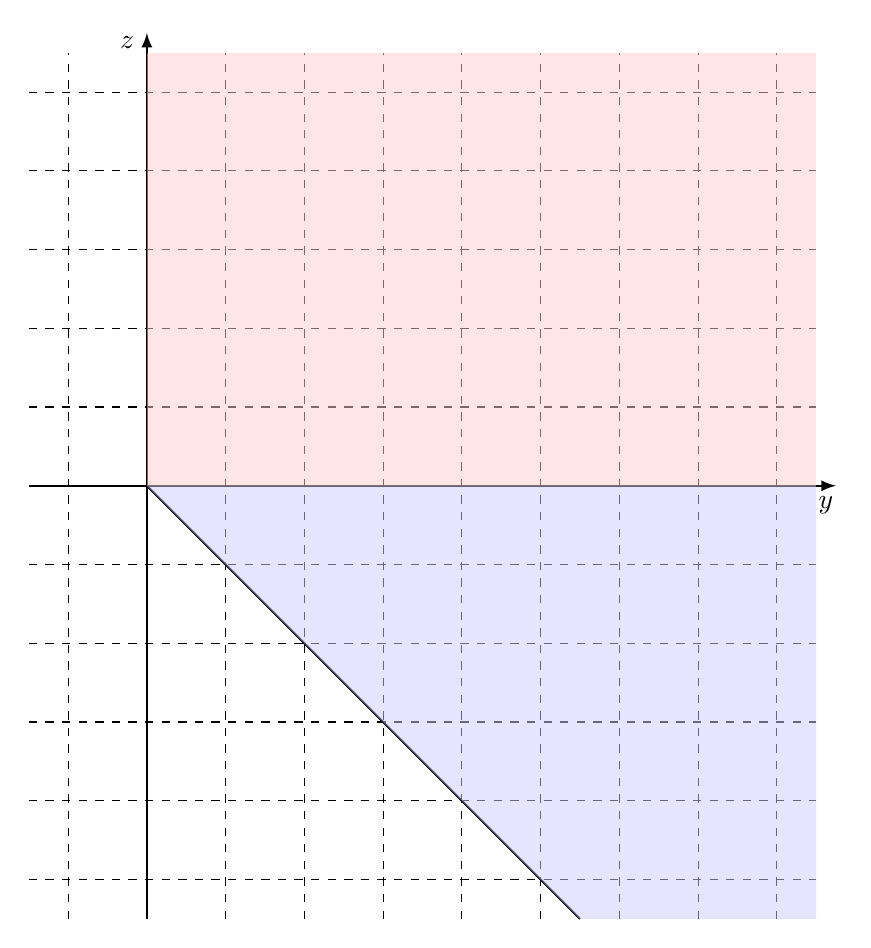
\begin{tikzpicture}
  \draw[-latex,thick] (-1.5,0) -- (8.75,0);
  \draw[-latex,thick] (0,-5.5) -- (0,5.75);
  \foreach \x in {-1,...,8}
    \draw[dashed] (\x,-5.5) -- (\x,5.5);
  \foreach \y in {-5,...,5}
    \draw[dashed] (-1.5,\y) -- (8.5,\y);

  
  \draw[thick] (0,0) -- (5.5,-5.5);
  \fill[color=blue!20,opacity=0.5] (0,0) -- (5.5,-5.5) -- (8.5,-5.5) -- (8.5,0) -- cycle;
  \fill[color=red!20,opacity=0.5]  (0,0) -- (0,5.5) -- (8.5,5.5) -- (8.5,0) -- cycle;

  \node at (-0.25,5.625) {$z$};
  \node at (8.625,-0.25) {$y$};

%  \draw[line width=0.6mm,blue] ( 2,0) -- ( 2,1);
%  \draw[line width=0.6mm,blue] ( 3,0) -- ( 3,2);
%  \draw[line width=0.6mm,blue] ( 4,0) -- ( 4,3);
%  \draw[line width=0.6mm,blue] ( 5,0) -- ( 5,4);
%  \draw[line width=0.6mm,blue] ( 6,0) -- ( 6,5);
%  \draw[line width=0.6mm,blue] ( 7,0) -- ( 7,6);
%  \draw[line width=0.6mm,blue] ( 8,0) -- ( 8,5);
%  \draw[line width=0.6mm,blue] ( 9,0) -- ( 9,4);
%  \draw[line width=0.6mm,blue] (10,0) -- (10,3);
%  \draw[line width=0.6mm,blue] (11,0) -- (11,2);
%  \draw[line width=0.6mm,blue] (12,0) -- (12,1);
%  
%  \foreach \x in {-1,...,13}
%    \node at (\x,-0.75) {\scriptsize \x};
%  \node[fill=white] at (-1.75,0) {\scriptsize 0};
%  \node[fill=white] at (-1.75,3) {\scriptsize 1/12};
%  \node[fill=white] at (-1.75,6) {\scriptsize 1/6};
\end{tikzpicture}
%%%
\caption{Domain of integration for the joint density function for the difference of two exponential distributions.}
\label{Fig:probability_differenceTwoExponentialDistributions}
\end{center}
\end{figure}

Since we are integrating over $y$ and the lower limit changes depending on whether $z < 0$ or $z \ge 0$, we break up the integral into two parts. For $z < 0$, the blue shaded are in Fig.~\ref{Fig:probability_differenceTwoExponentialDistributions}, the integral for the marginal density function is
\begin{align}
  f_{Z}(z) =  \int_{-z}^\infty \lambda \mu e^{-\lambda z} e^{-(\lambda + \mu) y } dy = \frac{\lambda \mu}{\lambda + \mu }e^{\mu z}, \quad z < 0.
\end{align}
For $z \ge 0$, the red shaded are in Fig.~\ref{Fig:probability_differenceTwoExponentialDistributions}, we have
\begin{align}
  f_{Z}(z) =  \int_0^\infty \lambda \mu e^{-\lambda z} e^{-(\lambda + \mu) y } dy = \frac{\lambda \mu}{\lambda + \mu }e^{-\lambda z}, \quad z \ge 0.
\end{align}
Pulling these two together, the probability density function is therefore given by the piecewise function
\begin{align}
  f_{Z}(z) = \left\{ \begin{array}{r l}
  \dfrac{\lambda \mu}{\lambda + \mu }e^{\mu z},      & \quad z < 0   \vspace{0.2cm} \\
  \dfrac{\lambda \mu}{\lambda + \mu }e^{-\lambda z}, & \quad z \ge 0 \vspace{0.2cm} \\ \end{array} \right. .
\end{align}
To find our desired probability, we integrate this over $z$ from $-\tau$ to $\tau$:
\begin{align}
  P( -\tau \le Z \le \tau ) &= \int_{-\tau}^0 \dfrac{\lambda \mu}{\lambda + \mu }e^{\mu z} dz + \int_0^{\tau} \dfrac{\lambda \mu}{\lambda + \mu }e^{-\lambda z} dz \nonumber \\*
  &= \frac{\lambda}{\lambda + \mu} ( 1 - e^{-\mu \tau} ) + \frac{\mu}{\lambda + \mu} ( 1 - e^{-\lambda \tau} ) \nonumber \\*
  &= 1 - \frac{ \lambda e^{-\mu \tau} + \mu e^{-\lambda \tau} }{ \lambda + \mu } .
\end{align}

%%%%%%%%%%%%%%%%%%%%%%%%%%%%%%%%%%%%%%%%%%%%%%%%%%%%%%%%%%%%%%%%%%%%%%%%%%%%%%%%%%%%%%%%%%%%%%%
\subsection{Products of Random Variables}

Another common operation for random variables is to take their product. Let $Z = XY$ where $X$ and $Y$ are (possibly dependent) random variables having joint probability density function $f_{X,Y}(x,y)$. As we did with the sum of random variables, we perform a transformation on either $X$ or $Y$. If we perform the let $y = z/x$, we have
\begin{align}
  \frac{dy}{dz} = -\frac{1}{x} ; \nonumber
\end{align}
therefore the joint density function for $X$ and $Z$ becomes
\begin{align}
  f_{X,Z}(x,z) = f_{X,Y}(x,y) \left| \frac{dy}{dz} \right| =  f_{X,Y}(x,z/x) \frac{1}{|x|}
\end{align}
The marginal density function in the product $Z$ may be obtained by integrating the joint density function over $x$:
\begin{align}
  f_Z(z) = \int_{-\infty}^\infty f_{X,Y}(x,z/x) \frac{dx}{|x|} .
\end{align}

%%%%%%%%%%%%%%%%%%%%%%%%%%%%%%%%%%%%%%%%%%%%%%%%%%%%%%%%%%%%%%%%%%%%%%%%%%%%%%%%%%%%%%%%%%%%%%%
%%%%%%%%%%%%%%%%%%%%%%%%%%%%%%%%%%%%%%%%%%%%%%%%%%%%%%%%%%%%%%%%%%%%%%%%%%%%%%%%%%%%%%%%%%%%%%%
\section{Error Propagation}

In performing experiments and collecting data, we often take the raw data and perform analysis by evaluating functions $g(X_1,X_2,\ldots)$. Unfortunately, there is always inherent randomness because of factors that are outside the control of the experimenters. We often do not have a detailed knowledge of how these variations in data from experimental results are distributed. Alternatively, we may have an understanding of the random distributions, but it is too difficult to calculate an exact random distribution for an arbitrary function $g(X_1,X_2,\ldots)$. For these cases, we approximate the mean and variance using error propagation formulas, which are based on Taylor series approximations. This section discusses the first-order Taylor series approximation and derives the error propagation formulas.


%%%%%%%%%%%%%%%%%%%%%%%%%%%%%%%%%%%%%%%%%%%%%%%%%%%%%%%%%%%%%%%%%%%%%%%%%%%%%%%%%%%%%%%%%%%%%%%
\subsection{First-Order Taylor Approximation}

To perform this analysis, let us consider the case of two random variables $X$ and $Y$ with a known measured sample means $\overline{x}$ and $\overline{y}$ respectively, sample variances $s_x^2$ and $s_y^2$ respectively, and correlation coefficient $\rho_{xy}$. The analysis will extend to any number of random variables, but using two simplifies the process. Now we introduce a new random variable $Z = g(X,Y)$ where we assume $g$ is a differentiable function that allows us to take a Taylor series expansion.

To begin, we perform a first-order Taylor series expansion of the random variable $Z$ about the sample means of $X$ and $Y$, $\overline{x}$ and $\overline{y}$ respectively:
\begin{align}
  z = g(x,y) \approx g(\overline{x},\overline{y}) + ( x - \overline{x} ) \dho{g}{x} + ( y - \overline{y} ) \dho{g}{y} .
\end{align}
Here the partial derivatives are taken to be evaluated at $(\overline{x},\overline{y})$. We then take the expectation of random variable $Z$:
\begin{align}
  E(Z) = \overline{z} \approx E( g(\overline{x},\overline{y}) ) + \dho{g}{x} ( E(X) - \overline{x} ) + \dho{g}{y} ( E(Y) - \overline{y} ) .
\end{align}
The first term is a non-random variable, so the expectation is itself. Our best estimate of the expectations are the sample means, $E(X) = \overline{x}$ and $E(Y) = \overline{y}$. Therefore, the second and third terms vanish, leaving us with the simple result:
\begin{align}
  E(Z) = \overline{z} \approx g(\overline{x},\overline{y}) .
\end{align}
To compute the variance, let us take the difference $Z - E(Z)$,
\begin{align}
  Z - E(Z) = z - \overline{z} = g(\overline{x},\overline{y}) + ( x - \overline{x} ) \dho{g}{x} + ( y - \overline{y} ) \dho{g}{y} - g(\overline{x},\overline{y})
\end{align}
The first and fourth terms cancel. Squaring the remaining two terms gives
\begin{align}
  ( Z - E(Z) )^2 &= ( z - \overline{z} )^2 \nonumber \\
  &= ( x - \overline{x} )^2 \left( \dho{g}{x} \right)^2 + ( y - \overline{y} )^2 \left( \dho{g}{y} \right)^2 \nonumber \\* 
  &\quad + 2 ( x - \overline{x} ) ( y - \overline{y} ) \left( \dho{g}{x} \right) \left( \dho{g}{y} \right) .
\end{align}
Taking the expectation gives
\begin{align}
  E[( Z - E(Z) )^2] &= s_z^2 = E[( x - \overline{x} )^2 ] \left( \dho{g}{x} \right)^2 + E[( y - \overline{y} )^2] \left( \dho{g}{y} \right)^2 \nonumber \\* 
  &\quad + 2 E[ ( x - \overline{x} ) ( y - \overline{y} ) ] \left( \dho{g}{x} \right) \left( \dho{g}{y} \right) . \nonumber
\end{align}
For the first and second terms, we recognize the expectations as the variances of random variables $X$ and $Y$ respectively, for which our best estimates are the respective sample variances $s_x^2$ and $s_y^2$. The third term is the covariance, which can be put in terms of the correlation coefficient as $\rho_{xy} s_x s_y$. This gives the first-order error propagation formula for two random variables:
\begin{align}
  s_z^2 = s_x^2 \left( \dho{g}{x} \right)^2 + s_y^2 \left( \dho{g}{y} \right)^2 
  + 2 \rho_{xy} s_x s_y \left( \dho{g}{x} \right) \left( \dho{g}{y} \right) . 
\end{align}

This result can be generalized to any number of random variables:
\begin{align}
  s_z^2 = \sum_{i=1}^N s_{x_i}^2  \left( \dho{g}{x_i} \right)^2 + 2 \sum_{j > i}^N \sum_{i=1}^N \rho_{ij} s_{x_i} s_{x_j}  \left( \dho{g}{x_i} \right)  \left( \dho{g}{x_j} \right) .
\end{align}
Equivalently if we have the sample covariance matrix $\boldsymbol\Sigma$ and the partial derivatives encoded in column vector $\mathbf{d}$ we can write this in matrix-vector form:
\begin{align}
  s_z^2 = \mathbf{d}^\top \boldsymbol\Sigma \mathbf{d}  .
\end{align}
This is often referred to as the \emph{sandwich rule} because it encloses the covariance matrix between two vectors of partial derivatives.

The first-order Taylor series is usually sufficient for most engineering applications with one major assumption. This assumption is that the function $g$ is sufficiently flat in the range of a few standard deviations that we can approximate it as a linear function. If $g$ is a rapidly varying function, a special case where the mean is at or near a critical point (where the derivatives would evaluate to zero), or if the variance is too large to make this assumption, then the first-order approximation is not particularly good and we may need to consider higher-order Taylor series expansions. The cost of doing this leads to very complicated systems of equations involving higher-order moments and correlations of the random variables, which may not be easy to measure in a statistically significant manner.

%%%%%%%%%%%%%%%%%%%%%%%%%%%%%%%%%%%%%%%%%%%%%%%%%%%%%%%%%%%%%%%%%%%%%%%%%%%%%%%%%%%%%%%%%%%%%%%
\subsection{Example: Attenuation of a Beam}

The equation for the attenuation of a beam without scattering is given as
\begin{align}
  I(x) = I_0 e^{-N \sigma x} .
\end{align}
This mathematical model is valid for a beam of low-energy ($< 100$~keV) photons on a high atomic-mass target such as lead or tungsten. Here $I_0$ is the initial intensity of the beam at $x = 0$, $N$ is the atomic density, $\sigma$ is the microscopic cross section, and $x$ is the depth into the target. 

We wish to understand the relative uncertainty, the ratio of the standard deviation to the expectation, of the beam intensity for various depths. To do this, we can apply the first-order Taylor series approximation to obtain the variance of the intensity. Here we assume the beam intensity $I_0$, atomic density $N$, and microscopic cross section $\sigma$ are uncertain parameters that are independent of each other. From the first-order Taylor series we can find the estimated variance of the intensity,
\begin{align}
  s_I^2 = s_{I_0}^2 \left( \dho{I}{I_0} \right)^2 + s_{N}^2 \left( \dho{I}{N} \right)^2 + s_{\sigma}^2 \left( \dho{I}{\sigma} \right)^2 .
\end{align}
The partial derivatives are
\begin{subequations}
\begin{align}
  \dho{I}{I_0}    &= e^{-N \sigma x}, \\
  \dho{I}{N}      &= I_0 \sigma x e^{-N \sigma x} , \\
  \dho{I}{\sigma} &= I_0 N x e^{-N \sigma x} .
\end{align}
\end{subequations}
Inserting these into the equation and factoring out the exponential, we have the variance of
\begin{align}
  s_I^2(x) = \left[  s_{I_0}^2 + ( I_0 \sigma x )^2 s_{N}^2 + ( I_0 N x )^2 s_{\sigma}^2 \right] e^{-2 N \sigma x} .
\end{align}
Taking the square root gives the standard deviation. If we then divide by $I(x)$ we then have the relative uncertainty as
\begin{align}
  R_I(x) = \frac{ s_I(x) }{ I(x) } = \dfrac{ \sqrt{ \left[  s_{I_0}^2 + ( I_0 \sigma x )^2 s_{N}^2 + ( I_0 N x )^2 s_{\sigma}^2 \right] } }{ I_0 } .
\end{align}
If we are given the following information:
\begin{align}
  I_0 &= 2 \times 10^8 \pm 1 \times 10^7 \text{ photons/s}, \nonumber \\*
  N   &= 0.05 \pm 0.001 \text{ atoms/b/cm}, \nonumber \\*
  \sigma &= 2 \pm 0.2 \text{ b} , \nonumber
\end{align}
then we can calculate
\begin{align}
  R_I(x) = \dfrac{ \sqrt{ \left[  ( 1 \times 10^{14} ) + ( 1.6 \times 10^{11} ) x^2 + ( 4 \times 10^{12} ) x^2  \right] } }{ I_0 } . \nonumber
\end{align}
Here each term corresponds to (from left to right) the contribution from the uncertainties in the initial beam intensity, the atom density, and nuclear cross section. We see that the term for uncertainty in the beam intensity has the largest magnitude, but the other two have a factor of $x^2$, which means the effect of the uncertainties in the atom density and nuclear cross section become more important with increasing depth. Of these two, the uncertainty in the nuclear cross section is more important.

%%%%%%%%%%%%%%%%%%%%%%%%%%%%%%%%%%%%%%%%%%%%%%%%%%%%%%%%%%%%%%%%%%%%%%%%%%%%%%%%%%%%%%%%%%%%%%%
\subsection{Linear Systems of Normally-Distributed Variables}

It is often the case that we have random variables that follow a normal distribution (or at least approximately so), which is often a consequence of the central limit theorem. We can show (with a good deal of math that is omitted) that the linear combination of normally distributed random variables is also normally distributed. This allows us to perform error propagation on these random variables without having to resort to performing convolution integrals or Taylor-series approximations.

Suppose we have the linear system of random variables:
\begin{align}
  Y_1 &= a_{1,1} X_1 + a_{1,2} X_2 + \cdots + a_{1,N} X_N, \nonumber \\
  Y_2 &= a_{2,1} X_1 + a_{2,2} X_2 + \cdots + a_{1,N} X_N, \nonumber \\
  &\vdots \nonumber \\
  Y_N &= a_{N,1} X_1 + a_{N,2} X_2 + \cdots + a_{N,N} X_N.
\end{align}
The random variables are all normally distributed with different mean values given by the column vector $\boldsymbol\mu_X$ and the covariance matrix $\boldsymbol\Sigma_X$. If the coefficients $a_{i,j}$ are stored in matrix $\mathbf{A}$ then the mean value of the $Y$ random variables are simply
\begin{align}
  \boldsymbol\mu_Y = \mathbf{A} \boldsymbol\mu_X .
\end{align}
The covariance matrix for the $Y$ random variables is given by
\begin{align}
  \boldsymbol\Sigma_Y = \mathbf{A}^\top \boldsymbol\Sigma_X \mathbf{A} .
\end{align}




%%%%%%%%%%%%%%%%%%%%%%%%%%%%%%%%%%%%%%%%%%%%%%%%%%%%%%%%%%%%%%%%%%%%%%%%%%%%%%%%%%%%%%%%%%%%%%%
%%%%%%%%%%%%%%%%%%%%%%%%%%%%%%%%%%%%%%%%%%%%%%%%%%%%%%%%%%%%%%%%%%%%%%%%%%%%%%%%%%%%%%%%%%%%%%%%
\section{Random Sampling}

In many applications the probability distributions are too complicated to analytically or even numerically evaluate on a computer. In these cases we perform random sampling of the underlying random or stochastic process. If we create numerous realizations of the stochastic process, we can then make inferences about its behavior. This is generally called the Monte Carlo method. Before we can discuss this approach, we need to develop techniques for sampling random variates from non-uniform distributions.

All major computer languages have the ability to generate random numbers from a uniform distribution. Often these random numbers are scaled to be in the range from 0 to 1 (with 1 often excluded). Using these sampled uniform random variables, called uniform variates with the symbol $\xi_i$ (or simply $\xi$ when we only are using a single uniform random variate), we are able to derive methods to find random variates from other distributions. The methods by which a computer generates uniform random variates are called pseudorandom number generation. The sequence of uniform variates are pseudorandom because they are usually generated using a deterministic algorithm; however, if we are given a sequence of these uniform variates, they will essentially appear uniformly random. This means that the sequence has no preference for any particular values in the range of 0 to 1 and there are no discernible patterns, i.e., if we do not know the underlying algorithm, simply knowing one random variate provides no information about the next random variate.

The process of generating random variates of non-uniform distributions is generally called random sampling. Textbooks have been written on this topic alone, so these notes can only cover the most basic techniques for generating random samples. Here we will discuss the methods of inversion and rejection sampling.

%%%%%%%%%%%%%%%%%%%%%%%%%%%%%%%%%%%%%%%%%%%%%%%%%%%%%%%%%%%%%%%%%%%%%%%%%%%%%%%%%%%%%%%%%%%%%%%
\subsection{Direct Inversion Sampling}

One approach for generating non-uniform random variates is called the direct inversion sampling method or simply the inversion method.

The inversion method proceeds by finding the cumulative distribution function of the random variable we wish to sample, call this $F_X(x)$. The cumulative distribution function, again, is a probability that a random variable $X$ is less than or equal to some value $x$. Since the cumulative distribution function is a probability, we know that it ranges from 0 to 1. We therefore equate the cumulative distribution function with a uniform variate $\xi$ and then solve for $x$. Formally, this is expressed as:
\begin{align}
  x = F^{-1}_X(\xi) .
\end{align}

To illustrate this, let us suppose that we wish to sample random variates of an exponential distribution with rate parameter $\lambda$. The reason for doing this may be to find the random time that a radioactive isotope undergoes decay or to find the random position that a particle undergoes an interaction with the background material. The cumulative density function is
\begin{align}
  F_X(x) = 1 - e^{-\lambda x } = \xi .
\end{align}
If we solve for $x$, we have
\begin{align}
  x = -\frac{1}{\lambda} \ln ( 1 - \xi ) .  \nonumber
\end{align}
We can make one more simplification and note that one minus a uniform random variable from 0 to 1 is still a uniform random variable from 0 to 1. Therefore, we can obtain a random sample from an exponential distribution using
\begin{align}
  x =  -\frac{1}{\lambda} \ln \xi .
\end{align}

A slightly more complicated example is the truncated exponential distribution with the probability density function
\begin{align}
  f_X(x) = \left\{ \begin{array}{r l}
  \dfrac{ \lambda e^{-\lambda x} }{ 1 - e^{-\lambda a } }, & \quad 0 \le x \le a  \vspace{0.2cm}  \\
  0,                                 & \quad \text{otherwise} \\ \end{array} \right. .
\end{align}
The cumulative distribution function is found by integrating from 0 to $x$, which gives
\begin{align}
  F_X(x) = \left\{ \begin{array}{r l}
  0,                                                  & \quad x < 0 \\
  \dfrac{ 1 - e^{-\lambda x} }{ 1 - e^{-\lambda a } }, & \quad 0 \le x \le a   \vspace{0.2cm} \\
  1,                                                  & \quad x > a \\ \end{array} \right. .
\end{align}
The range from $0 \le x \le a$ is the only portion of interest, so we set that equal to a uniform random variate,
\begin{align}
   \frac{ 1 - e^{-\lambda x} }{ 1 - e^{-\lambda a } } = \xi,
\end{align}
and solve for $x$, giving
\begin{align}
   x = -\frac{1}{\lambda} \ln \left[  1 - \xi ( 1 - e^{-\lambda a } ) \right] .
\end{align}
This equation is slightly more complicated than the previous form, largely because an extra factor of $1 - e^{-\lambda a }$, which was the one over the normalization constant.

The direct inversion sampling method is relatively straightforward in principle: obtain the cumulative distribution function, set it equal to a uniform variate, and solve for $x$. Unfortunately, only a limited number of random distributions have cumulative distribution functions that are analytically invertible. A common random distribution with a non-invertible cumulative distribution function is the normal distribution. For these distributions, we need to use other techniques.

%For example, the random variable with the probability density function
%\begin{align}
%  f_X(x) = \left\{ \begin{array}{r l}
%  \dfrac{ 1 + e^{-x} }{ 2 + e^{-1} }, & \quad 0 \le x \le 1    \\
%  0,                                 & \quad \text{otherwise} \\ \end{array} \right. 
%\end{align}
%yields the cumulative distribution function
%\begin{align}
%  F_X(x) = \left\{ \begin{array}{r l}
%  0,                                                  & \quad x < 0 \\
%  \dfrac{ 1 + x + \sinh(x) - \cosh(x) }{ 2 + e^{-1} }, & \quad 0 \le x \le 1    \\
%  1,                                                  & \quad x > 1 \\ \end{array} \right. 
%\end{align}
%Unfortunately, it is not possible to solve this cumulative distribution function for $x$ in a closed form. 

%%%%%%%%%%%%%%%%%%%%%%%%%%%%%%%%%%%%%%%%%%%%%%%%%%%%%%%%%%%%%%%%%%%%%%%%%%%%%%%%%%%%%%%%%%%%%%%
\subsection{Rejection Sampling}

If we have a random variable with a cumulative distribution function that cannot be inverted directly, a common approach to find random variates is to use the rejection sampling technique. 

The basic idea with rejection sampling is as follows: Suppose we wish to sample a random variable $X$ with probability density function $f_X(x)$. We take another distribution with a probability density function we know how to sample with probability density function $g_X(x)$ scaled by some constant $c > 1$ so that $c g_X(x) \ge f_X(x)$ for all $x$ in the domain of random variable $X$. We then sample a candidate value of $\hat{x}$ from $g_X(x)$ using, e.g., direct inversion. Next we decide whether to accept the candidate value $\hat{x}$. To do this, we sample a value $\hat{y}$ from a uniform distribution ranging from 0 to $c g_X(\hat{x})$. If the sampled value $\hat{y} \le f_X(\hat{x})$ we then accept $\hat{x} = x$. If it is not, we repeat the entire process until we are successful. Pseudocode for this algorithm is given in Fig.~\ref{Fig:probability_rejectionAlgorithm}.

\begin{figure}[tb!]
\begin{center}
\noindent \rule{\textwidth}{1pt}
\begin{verbatim}
 1. do until accept
 2.   sample x_hat from g(x)
 3.   xi = uniform random variate
 4.   y  = xi * c * g(xhat)
 5.   if y_hat <= f(x_hat)
 6.      accept x = x_hat
 7.   else
 8.      repeat loop
 9. return x
\end{verbatim}
\rule{\textwidth}{1pt}
\caption{Pseudocode for rejection sampling of $f_X(x)$ using $g_X(x)$.}
\label{Fig:probability_rejectionAlgorithm}
\end{center}
\end{figure}

One drawback with rejection sampling is that we may require numerous trials from sampling from $g_X(x)$ to obtain a valid sample of $f_X(x)$. Indeed, if $g_X(x)$ is not chosen carefully, we can end up with cases where we may spend a significant amount of time sampling $g_X(x)$ numerous times. We can calculate a sampling efficiency using the expectation:
\begin{align}
  \epsilon &= \int_{-\infty}^\infty \left[ \frac{ f_X(x) }{ c g_X(x) } \right] g_X(x) dx \nonumber \\
           &= \frac{1}{c} \int_{-\infty}^\infty f_X(x) dx = \frac{1}{c} .
\end{align}
Therefore, the sampling efficiency is inversely proportional to the scaling constant $c$ and this shows that we should select a distribution for which $c$ is smallest, i.e., a $g_X(x)$ that can tightly bound $f_X(x)$.

\begin{figure}[tb!]
\begin{center}
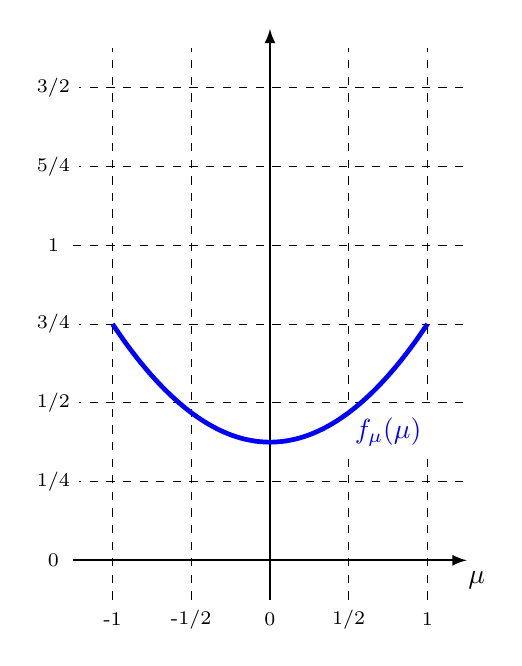
\begin{tikzpicture}
  \draw[-latex,thick] (-2.5,0) -- (2.5,0);
  \node at (2.625,-0.25) {$\mu$};
  \draw[-latex,thick] (0,-0.5) -- (0,6.75);
  \foreach \x in {-2,...,2}
    \draw[dashed] (\x,-0.5) -- (\x,6.5);
  \foreach \y in {0,...,6}
    \draw[dashed] (-2.5,\y) -- (2.5,\y);

  \node[color=blue,fill=white] at (1.5,1.625) {$f_\mu(\mu)$};

  \draw[line width=0.6mm,blue] plot[smooth,domain=-1:1] ({2*\x}, {4*3/8*( 1 + \x*\x )});

  \node[fill=white] at (-2.75,0) {\scriptsize 0};
  \node[fill=white] at (-2.75,1) {\scriptsize 1/4};
  \node[fill=white] at (-2.75,2) {\scriptsize 1/2};
  \node[fill=white] at (-2.75,3) {\scriptsize 3/4};
  \node[fill=white] at (-2.75,4) {\scriptsize 1};
  \node[fill=white] at (-2.75,5) {\scriptsize 5/4};
  \node[fill=white] at (-2.75,6) {\scriptsize 3/2};

  \node[fill=white] at (-2,-0.75) {\scriptsize -1};
  \node[fill=white] at (-1,-0.75) {\scriptsize -1/2};
  \node[fill=white] at ( 0,-0.75) {\scriptsize 0};
  \node[fill=white] at ( 1,-0.75) {\scriptsize 1/2};
  \node[fill=white] at ( 2,-0.75) {\scriptsize 1};
  
%  \draw[line width=0.6mm,blue] (-3,0) -- (0,2);
%  \draw[line width=0.6mm,blue] (0,2)  -- (6,0);
%  
%  \foreach \x in {-1,...,2}
%    \node at ({3*\x},-0.75) {\scriptsize \x};
%  \node[fill=white] at (-5.0,0) {\scriptsize 0};
%  \node[fill=white] at (-5.0,1) {\scriptsize 1/3};
%  \node[fill=white] at (-5.0,2) {\scriptsize 2/3};
%  \node[fill=white] at (-5.0,3) {\scriptsize 1};
\end{tikzpicture}
%%%
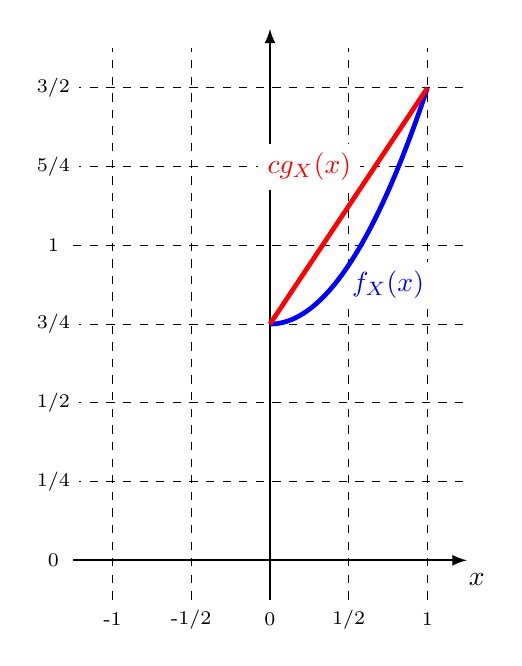
\begin{tikzpicture}
  \draw[-latex,thick] (-2.5,0) -- (2.5,0);
  \node at (2.625,-0.25) {$x$};
  \draw[-latex,thick] (0,-0.5) -- (0,6.75);
  \foreach \x in {-2,...,2}
    \draw[dashed] (\x,-0.5) -- (\x,6.5);
  \foreach \y in {0,...,6}
    \draw[dashed] (-2.5,\y) -- (2.5,\y);
    
  \node[color=blue,fill=white] at (1.5,3.5) {$f_X(x)$};
  \node[color=red, fill=white] at (0.5,5) {$c g_X(x)$};

  \draw[line width=0.6mm,blue] plot[smooth,domain=0:1] ({2*\x}, {4*3/4*( 1 + \x*\x )});
  \draw[line width=0.6mm,red] plot[smooth,domain=0:1] ({2*\x}, {4*3/4*( 1 + \x )});

  \node[fill=white] at (-2.75,0) {\scriptsize 0};
  \node[fill=white] at (-2.75,1) {\scriptsize 1/4};
  \node[fill=white] at (-2.75,2) {\scriptsize 1/2};
  \node[fill=white] at (-2.75,3) {\scriptsize 3/4};
  \node[fill=white] at (-2.75,4) {\scriptsize 1};
  \node[fill=white] at (-2.75,5) {\scriptsize 5/4};
  \node[fill=white] at (-2.75,6) {\scriptsize 3/2};

  \node[fill=white] at (-2,-0.75) {\scriptsize -1};
  \node[fill=white] at (-1,-0.75) {\scriptsize -1/2};
  \node[fill=white] at ( 0,-0.75) {\scriptsize 0};
  \node[fill=white] at ( 1,-0.75) {\scriptsize 1/2};
  \node[fill=white] at ( 2,-0.75) {\scriptsize 1};
  
  
%  \draw[line width=0.6mm,blue] (-3,0) -- (0,2);
%  \draw[line width=0.6mm,blue] (0,2)  -- (6,0);
%  
%  \foreach \x in {-1,...,2}
%    \node at ({3*\x},-0.75) {\scriptsize \x};
%  \node[fill=white] at (-5.0,0) {\scriptsize 0};
%  \node[fill=white] at (-5.0,1) {\scriptsize 1/3};
%  \node[fill=white] at (-5.0,2) {\scriptsize 2/3};
%  \node[fill=white] at (-5.0,3) {\scriptsize 1};
\end{tikzpicture}
\caption{Probability density function for scattering cosine $\mu$ of Rayleigh scattering (left) and illustration of rejection sampling of the half distribution using a linear bounding function (right).}
\label{Fig:probability_rejectionRayleighScatteringExample}
\end{center}
\end{figure}

As an example, let us consider Rayleigh scattering of photons. In Rayleigh scattering, a photon interacts with an atom and elastically scatters, changing direction, but maintaining its energy. The cosine of the angle between the incoming and outgoing photon velocity vectors is random because of the laws of quantum mechanics. The probability density function for the cosine of the scattering angle $\mu$ is
\begin{align}
  f_\mu(\mu) = \frac{3}{8} ( 1 + \mu^2 ), \quad -1 \le \mu \le 1 .
\end{align}
This probability density function is plotted on the left plot of Fig.~\ref{Fig:probability_rejectionRayleighScatteringExample}. It turns out this distribution yields an invertible cumulative density function, but the inversion process yields a very complicated expression. A better approach would be to apply rejection sampling.

To begin, we first note the Rayleigh scattering probability density function is symmetric about the $y$ axis. Therefore, we can sample the right half of the distribution, and then with a probability of $\tfrac{1}{2}$ flip the sign. Since we are only going to sample half of the distribution, we scale $f(\mu)$ by a factor of 2 to get
\begin{align}
  f_X(x) = 2 f_\mu(x = | \mu |) =  \frac{3}{4} ( 1 + x^2 ), \quad 0 \le x \le 1 .
\end{align}

Now, we have several choices to sample half of the parabola. One choice that is fairly straight-forward is to use a probability density function $g_X(x)$ as a line that connects the endpoints of the parabola from $f_X(x)$. This is
\begin{align}
  c g_X(x) = \frac{3}{4} ( 1 + x ) .
\end{align}
An illustration of $c g_X(x)$ with the probability density function $f_X(x)$ is displayed on the right plot in Fig.~\ref{Fig:probability_rejectionRayleighScatteringExample}. To find the value of $c$ and $g_X(x)$, we need a probability density function proportional to $1 + x$ from $0 \le x \le 1$. This can be found from
\begin{align}
  \int_0^1 A ( 1 + x ) dx = 1,
\end{align}
where $A$ is a normalization constant. If we carry out the integral, we can find that $A = \tfrac{2}{3}$ and have
\begin{align}
  g_X(x) = \frac{2}{3} ( 1 + x ) .
\end{align}
The constant is therefore $c = \tfrac{9}{8}$ implying the sampling efficiency is $\epsilon = \tfrac{8}{9} \approx 0.89$. Now, we seek to sample from $g_X(x)$ using direct inversion. To do this, we obtain the cumulative distribution function
\begin{align}
  G_X(x) = \int_0^x g_X(x') dx' = \frac{1}{3} ( x^2 + 2 x ) .
\end{align}
Setting this equal to a uniform variate $\xi_1$ yields the quadratic equation
\begin{align}
  x^2 + 2 x - 3 \xi_1 = 0.
\end{align}
Solving this and retaining the positive root gives our candidate value of
\begin{align}
  \hat{x} = \sqrt{ 3 \xi_1 + 1 } - 1 .
\end{align}
Next we sample our value of $\hat{y}$ using a new uniform random variate $\xi_2$,
\begin{align}
  \hat{y} = \xi_2 c g_X(\hat{x}) =  \frac{3 \xi_2}{4} ( 1 + \hat{x} ) .
\end{align}
Now we check if we have a successful sample of $f_X(x)$ if $\hat{y} \le f_X(\hat{x})$. This is
\begin{align}
  \xi_2 ( 1 + \hat{x} ) \le  1 + \hat{x}^2.
\end{align}
If we satisfy this condition, we let $x = \hat{x}$; if not, we repeat the process. Finally, we need find $\mu$ using the symmetry applied earlier. With probability $\tfrac{1}{2}$, $\mu = x$, and also with probability $\tfrac{1}{2}$, $\mu = -x$. To do this, we draw another uniform variate $\xi_3$ and set $\mu$ as 
\begin{align}
  \mu = \left\{ \begin{array}{r l}
   x, & \quad 0 \le \xi_3 < \frac{1}{2} \\
  -x, & \quad \tfrac{1}{2} \le \xi_3 < 1 \\ \end{array} \right. .
\end{align}


%%%%%%%%%%%%%%%%%%%%%%%%%%%%%%%%%%%%%%%%%%%%%%%%%%%%%%%%%%%%%%%%%%%%%%%%%%%%%%%%%%%%%%%%%%%%%%%
%%%%%%%%%%%%%%%%%%%%%%%%%%%%%%%%%%%%%%%%%%%%%%%%%%%%%%%%%%%%%%%%%%%%%%%%%%%%%%%%%%%%%%%%%%%%%%%%
\section{Monte Carlo Methods}

The Monte Carlo method describes a broad class of methods that are used to solve a variety of problems using random numbers. The method was originally developed shortly after the conclusion of the Second World War during the waning days of the Manhattan Project at Los Alamos to model the transport of radiation, which is a random process. Since the method has been applied in just about every quantitative discipline ranging from particle physics, evolutionary biology, economics, political science, and more. In this section, we will discuss Monte Carlo integration and its application to the transport of radiation through matter.

%%%%%%%%%%%%%%%%%%%%%%%%%%%%%%%%%%%%%%%%%%%%%%%%%%%%%%%%%%%%%%%%%%%%%%%%%%%%%%%%%%%%%%%%%%%%%%%
\subsection{Monte Carlo Integration}

It is often the case we encounter integrals that cannot be performed analytically. In these cases, we need to use numerical approximation schemes such as the trapezoid or Simpson's rule. The approach of breaking the integration domain into small intervals works well for one-dimensional integrals. However, it is often the case we need to evaluate multi-dimensional integrals and it can be computationally prohibitive to perform the integration. For example, in radiation transport, we are required to perform six-dimensional integrals: three spatial, two directional, and one energy. In solid state physics, we need to integrate probability density functions for the positions of all particles in a the element, which can range in the hundreds of dimensions. The statistical models encountered in social science or economics can have a similar dimensionality.

For high-dimensional integrals, it is simply impractical to perform the integration directly using standard numerical techniques. Fortunately, the Monte Carlo method can often be employed to make evaluating these integrals tractable. In this section, we will cover the one-dimensional case.

The idea is very similar to rejection sampling. Suppose we wish to evaluate the integral
\begin{align}
  \int_a^b f(x) dx, \nonumber
\end{align}
where $f(x)$ is some function satisfying $0 \le f(x) < \infty$ in the domain $a \le x \le b$. If we can find a probability density function $g_X(x)$ on the domain $a \le x \le b$ and a constant $c > 0$ such that $cg_X(x) \ge f(x)$ in the domain, we can evaluate the integral using rejection sampling via the sampling efficiency. The sampling efficiency is the expected number of samples that are accepted and is
\begin{align}
  \epsilon = \int_a^b \left[ \frac{ f(x) }{ c g_X(x) } \right] g_X(x) dx = \frac{1}{c} \int_a^b f(x) dx .
\end{align}
Therefore, the integral is
\begin{align}
   \int_a^b f(x) dx = c \epsilon.
\end{align}
The constant $c$ is determined by bounding $f(x)$ with $c g_X(x)$ and the sampling efficiency $\epsilon$ is determined using rejection sampling.

\begin{figure}[tb!]
\begin{center}
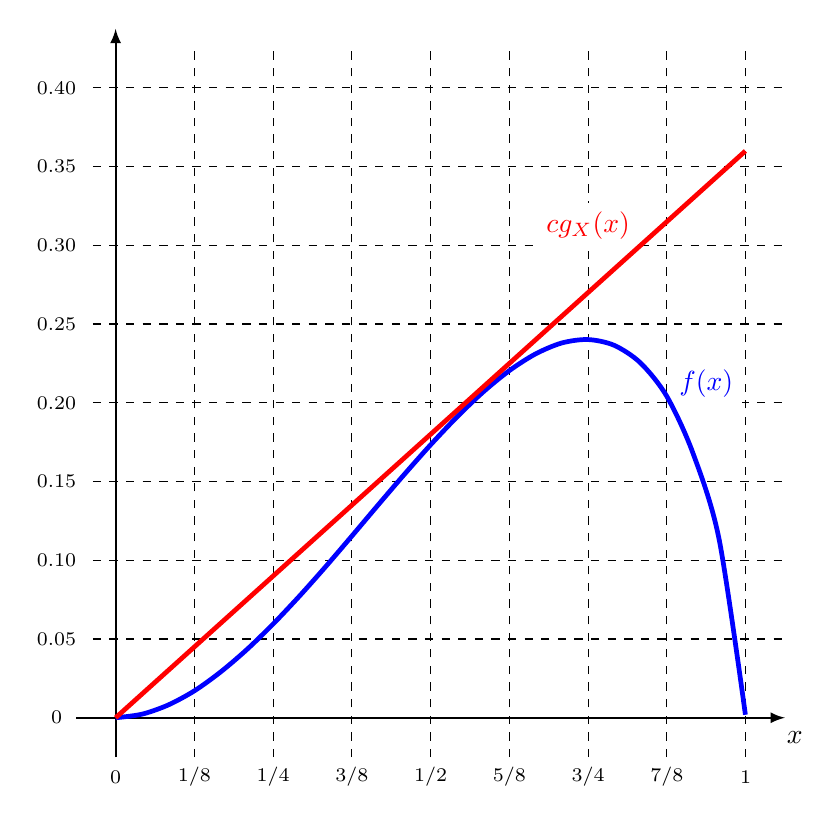
\begin{tikzpicture}
  \draw[-latex,thick] (-0.5,0) -- (8.5,0);
  \node at (8.625,-0.25) {$x$};
  \draw[-latex,thick] (0,-0.5) -- (0,8.75);
  \foreach \x in {0,...,8}
    \draw[dashed] (\x,-0.5) -- (\x,8.5);
  \foreach \y in {0,...,8}
    \draw[dashed] (-0.5,\y) -- (8.5,\y);


  \node[color=blue,fill=white] at (7.5,4.25) {$f(x)$};
  \node[color=red,fill=white]  at (6,6.25) {$cg_X(x)$};
%
  \draw[line width=0.6mm,blue] plot[smooth,domain=0:1] ({8*\x}, {20*(\x - 1)*ln( cos(deg(pi*\x/2)) )});
  \draw[line width=0.6mm,red]  plot[smooth,domain=0:1] ({8*\x}, {20*0.18*2*\x});

  \node[fill=white] at (-0.75,0) {\scriptsize 0};
  \node[fill=white] at (-0.75,1) {\scriptsize 0.05};
  \node[fill=white] at (-0.75,2) {\scriptsize 0.10};
  \node[fill=white] at (-0.75,3) {\scriptsize 0.15};
  \node[fill=white] at (-0.75,4) {\scriptsize 0.20};
  \node[fill=white] at (-0.75,5) {\scriptsize 0.25};
  \node[fill=white] at (-0.75,6) {\scriptsize 0.30};
  \node[fill=white] at (-0.75,7) {\scriptsize 0.35};
  \node[fill=white] at (-0.75,8) {\scriptsize 0.40};

  \node[fill=white] at ( 0,-0.75) {\scriptsize 0};
  \node[fill=white] at ( 1,-0.75) {\scriptsize 1/8};
  \node[fill=white] at ( 2,-0.75) {\scriptsize 1/4};
  \node[fill=white] at ( 3,-0.75) {\scriptsize 3/8};
  \node[fill=white] at ( 4,-0.75) {\scriptsize 1/2};
  \node[fill=white] at ( 5,-0.75) {\scriptsize 5/8};
  \node[fill=white] at ( 6,-0.75) {\scriptsize 3/4};
  \node[fill=white] at ( 7,-0.75) {\scriptsize 7/8};
  \node[fill=white] at ( 8,-0.75) {\scriptsize 1};
\end{tikzpicture}
\caption{Example for Monte Carlo integration.}
\label{Fig:probability_monteCarloIntegrationExample}
\end{center}
\end{figure}

As an example, suppose we wish to evaluate the integral
\begin{align}
  I = \int_0^1 ( x - 1 ) \ln \left[ \cos \left( \frac{\pi x}{2} \right) \right] dx.
\end{align}
This integral does not have any result in terms of standard (non-special) functions. Since this is a single integral, we could perform this integral using numerical techniques without too much trouble and get the result of approximately 0.133434; however, we will also use Monte Carlo integration to illustrate the concept. 

A plot of $f(x)$ is given by the blue curve in Fig.~\ref{Fig:probability_monteCarloIntegrationExample}. From this curve, it appears that we could reasonably bound this with a linear function as we did in the previous rejection sampling example for Rayleigh scattering. The probability density function is
\begin{align}
  g_X(x) = 2x, \quad 0 \le x \le 1 ,
\end{align}
which may be sampled using direct inversion. The cumulative density function is
\begin{align}
  G_X(x) = x.
\end{align}
Setting this equal to a uniform variate and solving, gives the sampling scheme
\begin{align}
  x = \sqrt{ \xi } .
\end{align}
Using graphical methods, we plot $g_X(x)$ scaled by a constant $c$ and determine that $c = 0.18$ appears to allow us to bound $f(x)$ with $c g_X(x)$ tightly. For illustration, the function $cg_X(x)$ is plotted using the red line in Fig.~\ref{Fig:probability_monteCarloIntegrationExample}.

\begin{table}[t!]
\caption{Monte Carlo Integration Results of $(x-1)\ln( \cos( \pi x / 2 ) )$ from 0 to 1}
\begin{center}
\begin{tabular}{|c|c|} \hline
$N$    & $I$      \\ \hline
$10^3$ & 0.135    \\
$10^4$ & 0.132912 \\
$10^5$ & 0.133411 \\
$10^6$ & 0.133398 \\
$10^7$ & 0.133416 \\
$10^8$ & 0.133443 \\ \hline
Numerical & 0.133434 \\ \hline
\end{tabular}
\end{center}
\label{Table:probability_monteCarloIntegrationExampleResults}
\end{table}%

Using the rejection method for $N$ random samples from $g_X(x)$, we tabulate the sampling efficiency and multiply the result by $c = 0.18$ to get an approximate value of the integral. Table~\ref{Table:probability_monteCarloIntegrationExampleResults} gives a list of numerical results for various sample sizes ranging from $10^3$ to $10^8$ compared to the reference result obtained using numerical integration. The results converge as the sample size increases with a convergence rate of $1/\sqrt{N}$ by way of the central limit theorem.


%%%%%%%%%%%%%%%%%%%%%%%%%%%%%%%%%%%%%%%%%%%%%%%%%%%%%%%%%%%%%%%%%%%%%%%%%%%%%%%%%%%%%%%%%%%%%%%
\subsection{Application to Particle Transport}

A common application of the Monte Carlo method is to simulate the transport of radiation particles. From these simulations, we can estimate quantities of interest that are describable through integrals of the function describing the average behavior of the radiation field. The behavior of individual particles is inherently random because of the laws of quantum mechanics; however, the collective behavior of large numbers of particles tends toward a deterministic function as the number gets large. For many applications, we are only concerned with the average behavior of particle behavior, and this section will cover this case. The Monte Carlo method is powerful in that it can also inform us about random statistical fluctuations in the radiation field as well, but this topic will not be covered here. Additionally, here we will discuss the transport of neutral particles only (e.g., neutrons and photons).

To begin, we introduce the concept of a \emph{particle history}. A particle history is a sequence of events spanning the birth of the particle to the removal of that particle and any other particles it may have created during that history (e.g., through nuclear fission). The Monte Carlo particle transport simulation performs numerous random particle histories. During these histories, information about physical quantities of interest is extracted and put into an accumulator to compute average values of physical quantities.

The first step in any particle history is to create the source particle. For this, we must be provided a source distribution $Q(\pos,\dir,E,t)$ where $\pos$ is the position, $\dir$ is a unit vector describing the particle direction, $E$ is the kinetic energy of the particle, and $t$ is the time that it is emitted. We then normalize $Q(\pos,\dir,E,t)$ and use random sampling techniques to find the random starting location of the particle.

After a particle is emitted, the particle will move until it interacts with a background atom/nucleus or transits into another region. The distance to particle interaction is proportional to the macroscopic total cross section or attenuation coefficient $\Sigma_t(E)$ in the current region. The distance to interaction or collision is given by an exponential distribution and found using direct inversion as
\begin{align}
  \ell_c = -\frac{1}{\Sigma_t(E)} \ln \xi .
\end{align}

We then calculate the distance that the particle would travel until it crosses into the adjacent region or edge of the problem, call this $\ell_s$. The distance to surface crossing is a deterministic, or non-random, quantity given a starting position $\pos$ and direction $\dir$. Most often, we describe the surfaces in a Monte Carlo particle transport equation using analytic equations. For example, a plane has the equation
\begin{align}
  S(x,y,z) = A x + B y + C z - D = 0,
\end{align}
where $A$, $B$, $C$, and $D$ are coefficients that determine the orientation of the plane. To find the distance we set each coordinate to the point at the surface point $x \rightarrow x + \Omega_x \ell_s$, $y \rightarrow y + \Omega_y \ell_s$, $z \rightarrow z + \Omega_z \ell_s$ and then solve for $\ell_s$. Here $(x,y,z)$ are the particle positions at the start of the trajectory and $(\Omega_x,\Omega_y,\Omega_z)$ are components of the unit direction vector of the particle. For the plane this is
\begin{align}
  A ( x + \Omega_x \ell_s ) + B ( y + \Omega_y \ell_s ) + C ( z + \Omega_z \ell_s ) - D = 0.
\end{align}
Solving this gives the distance to the plane as
\begin{align}
  \ell_s = \frac{ D - A x - B y - C z }{ A \Omega_x + B \Omega_y + C \Omega_z } .
\end{align}
If we get a negative value for $\ell_s$, then that means the particle is traveling away from the plane and we throw out the distance as not a possible intersection point.

Another common surface is a sphere at the origin, which has the equation
\begin{align}
  S(x,y,z) = x^2 + y^2 + z^2 - R^2 = 0,
\end{align}
with $R$ being the radius. As with the plane, we get the equation for the distance $\ell_s$ as
\begin{align}
  S(x,y,z) = ( x + \Omega_x \ell_s )^2 + ( y + \Omega_y \ell_s )^2 + ( z + \Omega_z \ell_s )^2 - R^2 = 0,
\end{align}
We can rewrite this as a quadratic equation for $\ell_s$ as
\begin{align}
  \ell_s^2 + 2 ( x \Omega_x + y \Omega_y + z \Omega_z  ) \ell_s +  \left( x^2 + y^2 + z^2  - R^2 \right) = 0 .
\end{align}
We can then solve this quadratic equation to obtain its two roots. The value of $\ell_s$ is the smallest positive, real root. If we have two positive roots, then the particle is entering the surface and will intersect twice. We take the smallest, as it is the next intersection point. Finding a positive and negative root implies that the particle is inside the surface and the positive root gives the distance until it leaves, whereas the negative root is the distance in the opposite direction. Having two negative roots implies the particle is outside the sphere and moving away from it. Finally, complex roots imply that the particle will not enter the surface at all. In all these cases, except for the smallest positive root, we eliminate those roots from consideration.

To decide which surface the particle intersections, we calculate the distances to all valid surfaces and take the smallest positive distance. This gives us the distance to surface $\ell_s$.

\begin{figure}[tb!]
\begin{center}
\noindent \rule{\textwidth}{1pt}
\begin{verbatim}
 1. dist to collision = -log(rand)/sigma_t
 2. dist to surface   = infinity
 3. loop over surfaces bounding region:
 4.   candiate dist = solution to surface equation
 5.   if candidate dist > 0:
 6.     dist to surface = min( dist to surface, candidate dist )
 7. dist to next event = min( dist to collision, dist to surface )
\end{verbatim}
\rule{\textwidth}{1pt}
\caption{Pseudocode for finding the distance to the next event in Monte Carlo particle transport.}
\label{Fig:probability_monteCarloTransportTrackingAlgorithm}
\end{center}
\end{figure}


Next, given $\ell_c$ and $\ell_s$ we need to determine the next event for the particle by taking the smallest of the two. To summarize this, pseudocode for calculating the distance to the next event is given in Fig.~\ref{Fig:probability_monteCarloTransportTrackingAlgorithm}.

If $\ell_s$ is smaller, we advance the particle to the adjacent region by moving the particle a distance $\ell_s$ along its direction $\dir$. If the particle reaches the edge of the problem, we stop that particle trajectory. If there is another adjacent region, we randomly sample a new distance to collision, calculate a new distance to intersecting surface, and determine the next event. If $\ell_c$ is smaller, we then advance the particle a distance $\ell_c$ along its direction $\dir$ and then we randomly determine the result of the collision, which is a random process because of the laws of quantum mechanics.

To process the random collision, first we need to determine the atom or nuclide that the particle interacts with. Each of these atoms/nuclides has an index $j$ and has its own total macroscopic cross section or interaction coefficient $\Sigma_t^j(E)$ (note that $j$ is a superscript, not a power) such that the total interaction coefficient for the material is
\begin{align}
  \Sigma_t(E) = \sum_{j=1}^J \Sigma_t^j(E) .
\end{align}
We can use these total interaction coefficients to construct a probability mass and cumulative distribution function for the random atom/nuclide. The probability that the particle interacts with a particular atom/nuclide $j$ is
\begin{align}
  p_j = \frac{ \Sigma_t^j(E) }{ \Sigma_t(E) } .
\end{align}
To find this, we construct a cumulative distribution function, get a new uniform random variate $\xi$, and determine the range that it is within.

Once we have determined the atom or nuclide $j$, we have to determine the reaction type. The conditional probability that a specific type of reaction $r$ with atom/nuclide $j$ given that a collision with atom/nuclide $j$ occurs is
\begin{align}
  p_r^j = \frac{ \Sigma_r^j(E) }{ \Sigma_t^j(E) } .
\end{align}
In the exact same manner as randomly sampling the atom or nuclide, we construct a cumulative distribution, draw another different uniform random variate, and find where it falls to determine the reaction. A detailed algorithm of sampling the atom/nuclide and the reaction is given in Fig.~\ref{Fig:probability_monteCarloTransportReactionSamplingAlgorithm}.

\begin{figure}[tb!]
\begin{center}
\noindent \rule{\textwidth}{1pt}
\begin{verbatim}
 1. r1 = rand
 2. s1 = 0
 3. loop j over all atoms/nuclides:
 4.   s1 += total xs for atom/nuclide j
 5.   if r1 < s1 * total xs for material:
 6.     select atom/nuclide j
 7.     exit loop
 8. r2 = rand
 9. s2 = 0
10. loop k over all reactions in atom/nuclide j:
11.   s2 += xs for reaction k of atom/nuclide j
12.   if r2 < s2 * total xs for atom/nuclide j:
13.     select reaction k
14.     exit loop
\end{verbatim}
\rule{\textwidth}{1pt}
\caption{Pseudocode for sampling the atom/nuclide and corresponding reaction.}
\label{Fig:probability_monteCarloTransportReactionSamplingAlgorithm}
\end{center}
\end{figure}

Depending on the particle type and the atom or nuclide, there are numerous possible types of reactions that may be possible. For neutrons, the common reactions are capture, elastic scattering, and fission. For photons, we have as common reactions as photoelectric absorption, Compton (incoherent elastic) scattering, and pair production. We then discuss the general idea for handling each of those cases.

For the capture or photoelectric absorption reactions, the neutron or photon respectively disappears. In the case of neutron capture, the resulting nucleus is usually in an excited state and the de-excitation leads to the emission of one or more photons. These photons are then stored and continue in the current history. Likewise, photoelectric effect can lead to the emission of fluorescence x-ray photons that may need to be followed. Additionally, the ejected electron can create lower-energy Bremsstrahlung photons. Depending on the level of fidelity desired, these secondary photons may or may not be tracked. In this section, we will ignore these secondaries.

In elastic scattering events, we are given a continuous probability density function for $\mu_0$, which is the cosine of the angle between the incident and outgoing photon direction vectors. We sample a $\mu_0$ from the probability density function $f_{\mu_0}(\mu_0)$ and then compute the outgoing direction vector using a 3-D rotation matrix. Going through this process is beyond the scope of these notes. For lower energy photons ($< 100$~keV) or lower energy neutrons scattering off of heavy targets (e.g., $< 100$~keV off of uranium), however, we may assume that scattering is isotropic or equiprobable in all directions. In this case, we sample the polar cosine uniformly from -1 to 1 using
\begin{subequations}
\begin{align}
  \mu_0 = 2 \xi_1 - 1,
\end{align}
and an azimuthal angle uniformly from 0 to $2\pi$ using
\begin{align}
  \gamma_0 = 2 \pi \xi_2 .
\end{align}
\end{subequations}
The outgoing direction vector components are the spherical coordinates with unit radius written as
\begin{subequations}
\begin{align}
  \Omega_x &= \sqrt{ 1 - \mu_0^2 } \cos \gamma_0, \\
  \Omega_y &= \sqrt{ 1 - \mu_0^2 } \sin \gamma_0, \\
  \Omega_z &= \mu_0 .
\end{align}
\end{subequations}
The outgoing kinetic energy is determined from conservation of momentum and mechanical energy.

In pair production, the original photon is destroyed and two photons are emitted with a kinetic energy of $m_e c^2 = 0.511$~MeV. The direction $\dir$ of one of the photons is sampled isotropically using the method described for isotropic elastic scattering. The second photon is given a direction in the opposite direction $-\dir$ and is stored for later on in the history after the first photon is removed from the problem.

For nuclear fission, the original neutron is absorbed and we have a random number of neutrons emitted each isotropically and at random energies. For the number of neutrons emitted, e.g., the multiplicity, we rarely have a reliably-measured probability mass function for the multiplicity that we can sample. Rather, we are usually only provided the mean value $\overline{\nu}$, which is a non-integer quantity. In this case, the best we can do is sample the multiplicity in a way that preserves this average. There are infinitely many ways one could do this, but a simple approach uses the distribution
\begin{align}
  \nu  = \left\lfloor \overline{\nu} + \xi \right\rfloor ,
\end{align}
where $\lfloor \cdot \rfloor$ is the ``floor'' operator that rounds down to the nearest integer. For example if $\overline{\nu} = 2.6$, then with probability 0.4 we will have $\nu = 2$ neutrons emitted, and probability 0.6 we will have $\nu = 3$ neutrons emitted with the average coming out to 2.6. For each neutron, we independently sample a direction isotropically and an outgoing energy from some provided distribution $f(E)$ often given the symbol $\chi(E)$. All but one of these particles are stored in a bank for later in the same history with the last one continuing the history.

After the collision is processed, if we have a surviving particle, the history continues by sampling a new distance to collision and calculating a new distance to surface. The particle keeps going until it is absorbed or leaks out of the problem. At this point, we look to see if we have any stored particles in a bank of particles. If there are, the history continues using by taking one of these stored particles out of the bank and executing the particle transport routines on it. Once the bank is fully depleted and no particles remain, the history terminates. The calculation continues with the next history until all the number of particle histories have been performed, at which point the calculation stops and results are provided to the user.

In terms of getting results, we keep track of accumulators called estimators or tallies that are ``scored'' during the particle histories. The most common physical quantities to be estimated are the particle scalar flux or path-length density or the particle current. The scalar flux or path-length density is used to calculate reaction rates, heating rates, biological dose, etc. As the name implies, the path-length density is the amount of path per unit volume the particles generate in a given history. For each region that we wish to know the scalar flux or path-length density, we get an estimate for that history $i$ as
\begin{align}
  \phi_i = \frac{1}{V} \sum_{\textrm{tracks} k} \ell_k ,
\end{align}
where $V$ is the volume of the region, $k$ is the index for the track in that region, and $\ell_k$ is the length of the track. This estimate can be multiplied by a response function $r(E)$ (e.g., cross section or flux to biological dose conversion factor) to get a reaction rate, dose, etc. by
\begin{align}
  R_i = \frac{1}{V} \sum_{\textrm{tracks } k} r_k(E) \ell_k ,
\end{align}
where $r_k(E)$ is the response function for the $k$th track. The particle current is simply the rate that particles cross a surface, which is obtained by counting up the number of surface crossings. The particle current is used in in applications where we, for example, wish to understand the effectiveness of a radiation shield. The particle current for history $i$ is
\begin{align}
  J_i = \sum_{\textrm{crossings } k} 1,
\end{align}
where $k$ in this context denotes the $k$th time a particle has crossed the surface in this history. At the end of the history, these estimates are added to a running sum and the average over $N$ histories is taken. For example, the scalar flux or path-length density is simply the sample mean
\begin{align}
  \phi = \frac{1}{N} \sum_{i=1}^N \phi_i ,
\end{align}
and likewise for any other response.

\begin{figure}[tb!]
\begin{center}
\noindent \rule{\textwidth}{1pt}
\begin{verbatim}
 1. loop i over number of histories:
 2.   draw starting particles from source distribution
 3.   insert source particles into back
 4.   while bank not empty:
 5.     pull particle out of bank
 6.     while particle alive:
 5.       sample random distance to collision dc
 6.       calculate distance to surface intersection ds
 7.       distance = min( dc, ds )
 8.       move particle by distance along path
 9.       compute scalar flux contribution along path
10.       if dc <= ds:        
11.         select nuclide and reaction
12.         process selected reaction (possibly kill particle)
13.         put secondaries in particle bank
14.       else:
15.         compute particle current contribution
16.         determine next region
17.         kill particle if exited problem
18.   add scalar flux and current estimators to accumulator   
19. divide accumulators by number of histories, write results
\end{verbatim}
\rule{\textwidth}{1pt}
\caption{Pseudocode for the overall Monte Carlo particle transport.}
\label{Fig:probability_monteCarloTransportAlgorithm}
\end{center}
\end{figure}

To summarize all of this discussion, the pseudocode for the overall Monte Carlo particle transport algorithm is given in Fig.~\ref{Fig:probability_monteCarloTransportAlgorithm}.







